\documentclass[francais]{rapport-leti}
%%%% PAQUETAGES %%%%
%\usepackage[T1]{fontenc}
\usepackage{t1enc}
\usepackage[latin1]{inputenc}
\usepackage{fancyhdr}
\usepackage{verbatim}
\usepackage{lastpage}
\usepackage{amsmath}
\usepackage{amssymb} 
\usepackage{graphicx}
\usepackage{color}
\usepackage{fancybox}
\usepackage{moreverb}
%\usepackage{hangcaption}
\usepackage[french]{babel}
%\selectlanguage{english}
\usepackage{csquotes}
%\usepackage[style=numeric-comp]{biblatex}
\usepackage{listings}
\usepackage{tikz}
\usetikzlibrary{shapes}
\usetikzlibrary{shapes.symbols}
\usetikzlibrary{decorations.pathreplacing}
\usepackage{hyperref}
\usepackage{subfigure}
\usepackage[font=small,labelfont=bf]{caption}

\usepackage{geometry}
\geometry{hmargin = 3.0cm, vmargin=2.9cm}

\usepackage{multirow}
\usepackage{xcolor,colortbl}


%%%% CONFIGURATION PAQUETAGES %%%%

\newtheorem{example}{Example}{\itshape}{\rmfamily}

%% Listings
\lstdefinestyle{customc}{
  belowcaptionskip=1\baselineskip,
  breaklines=true,
  frame=L,
  xleftmargin=\parindent,
  language=C,
  showstringspaces=false,
  basicstyle=\footnotesize\ttfamily,
  keywordstyle=\bfseries\color{green!40!black},
  commentstyle=\itshape\color{purple!40!black},
  identifierstyle=\color{blue},
  stringstyle=\color{orange},
}

\lstdefinestyle{customasm}{
  belowcaptionskip=1\baselineskip,
  frame=L,
  xleftmargin=\parindent,
  language=[x86masm]Assembler,
  basicstyle=\footnotesize\ttfamily,
  commentstyle=\itshape\color{purple!40!black},
}

\lstset{ numbers=left, tabsize=3, frame=single, numberstyle=\ttfamily,
basicstyle=\footnotesize, escapechar=@,style=customc,
           captionpos=b, % sets the caption position to bottom
               extendedchars=false, % for babel compatibility
}

%%% Hyperref
%\hypersetup{%
%    pdfborder = {0 0 0}
%}

%%% Styles
\fancypagestyle{normal}{
\fancyfoot[R]{
    \vspace{-2mm}
    \fontsize{10pt}{10pt}\selectfont
    \thepage /\pageref{LastPage}
    }
}


\fancypagestyle{plain}{
    \fancyhead{}
    \renewcommand{\headrulewidth}{0pt}
    \fancyfoot[R]{}
}


\fancypagestyle{append}{
    \fancyhead{}
    %\fancyhead[LE, RO]{ANNEXE~\thesection}
    \fancyfoot[R]{
        \vspace{-2mm}
        \fontsize{10pt}{10pt}\selectfont
            \thepage /\pageref{LastPage}}
}

%% Bibliographie
%\bibliography{my_bib}
%\DefineBibliographyStrings{french} {
%    urlseen = {consulté le},
%}

\makeatletter
\newcommand{\@givenstar}[2]{#1\;\middle|\;#2}
\newcommand{\@givennostar}[3][]{#1#2\;#1|\;#3#1}
\newcommand{\given}{\@ifstar\@givenstar\@givennostar}
\makeatother

\DeclareMathOperator*{\argmin}{argmin}
\DeclareMathOperator*{\argmax}{argmax}

\def\etal{\textit{et al.} }
\newcommand {\ie}{{\em i.e.} }
\def\eg{\textit{e.g.} }
\def\via{\textit{via} }
\def\resp{{\em resp.} }
\def\th{$^\text{th}$}


\usepackage{tikz}
\usetikzlibrary{mindmap,backgrounds}
\usetikzlibrary{shapes}
\usetikzlibrary{shapes.symbols}
\usetikzlibrary{decorations.pathreplacing}
\usetikzlibrary{decorations.markings}
\usetikzlibrary{arrows}
\usetikzlibrary{patterns}
\usetikzlibrary{calc}
\usetikzlibrary{positioning}
\usetikzlibrary{matrix}



\newtheorem{assumption}{Assumption}{\bfseries}{\itshape}
%----------------------------------------------------------------------------------------
%	MY NOTATIONS
%----------------------------------------------------------------------------------------
\newcommand*{\vLeak}{x}
\newcommand*{\vLeakVec}{\vec{x}}
\newcommand*{\vaLeak}{X}
\newcommand*{\setLeak}{\vec{\mathcal{X}}}
\newcommand*{\vaLeakVec}{\vec{X}}
\newcommand{\setLeakTrain}{\setLeak_{\text{train}}}
\newcommand{\setLeakTest}{\setLeak_{\text{test}}}
\newcommand{\setLeakValidation}{\setLeak_{\text{validation}}}
\newcommand{\setLeakProfiling}{\setLeak_{\text{profiling}}}
\newcommand{\setTargetTrain}{\setTarget_{\text{train}}}
\newcommand{\setTargetTest}{\setTarget_{\text{test}}}
\newcommand{\setTargetValidation}{\setTarget_{\text{validation}}}
\newcommand{\setTargetProfiling}{\setTarget_{\text{profiling}}}

\newcommand*{\vNNOutput}{\ensuremath {\vec{y}}}

\newcommand*{\setData}{\mathcal{D}}
\newcommand*{\sizeSetData}{\lvert\setData\rvert}
\newcommand*{\setDataTrain}{\mathcal{D}_{\text{train}}}
\newcommand*{\setDataTest}{\mathcal{D}_{\text{test}}}
\newcommand*{\setDataValidation}{\mathcal{D}_{\text{validation}}}
\newcommand*{\setDataProfiling}{\mathcal{D}_{\text{profiling}}}
\newcommand*{\setDataAttack}{\mathcal{D}_{\text{attack}}}
\newcommand*{\setTarget}{\mathcal{Y}}
%\newcommand*{\setDataKDA}{\mathcal{D}_{\text{KDA}}}
%\newcommand{\setLeakKDA}{\setLeak_{\text{KDA}}}
%\newcommand{\setTargetKDA}{\setTarget_{\text{KDA}}}


\newcommand*{\sPOI}{\tau} %signal strength


\newcommand*{\publicParRandVar}{E}
\newcommand*{\publicParVar}{e}
\newcommand*{\keyRandVar}{K}
\newcommand*{\keyVar}{k}
\newcommand*{\keyStar}{k^\star}
\newcommand*{\keyVarSet}{\mathcal{K}}
\newcommand*{\sensVar}{z}
\newcommand*{\sensRandVar}{Z}
\newcommand*{\sensVarValue}[1]{s_{#1}}
\newcommand*{\sensVarGenValue}{s}
\newcommand*{\sensVarOneHot}[1]{\vec{s_{#1}}}
\newcommand*{\sensVarSet}{\mathcal{Z}}
\newcommand*{\numClasses}{\lvert\sensVarSet\rvert}
\newcommand*{\nbClasses}{\lvert\sensVarSet\rvert}
\newcommand*{\sensFunction}{f}
\newcommand{\featureSpace}{\mathcal{F}}
\newcommand*{\distinguisher}{\Delta}


\newcommand*{\yyy}{\vec{y}}
\newcommand*{\YYY}{\vec{Y}}
\newcommand*{\www}{\vec{w}}
%\newcommand*{\WWW}{\textbf{W}}
\newcommand*{\vvv}{\vec{v}}
%\newcommand*{\VVV}{\textbf{V}}

\newcommand*{\nbTraces}{N}
\newcommand*{\nbTrainingTraces}{N_t}
\newcommand*{\nbProfilingTraces}{N_p}
\newcommand*{\nbProfilingTracesPerClass}{N_{p,\sensVarGenValue}}
\newcommand*{\nbAttackTraces}{N_a}
\newcommand*{\nbTracesPerClass}[1][\sensVarGenValue]{N_{#1}}
\newcommand*{\guessingEntropy}{\mathrm{GE}}
\newcommand*{\SR}{\mathrm{SR}}
\newcommand*{\newTraceLength}{C}
\newcommand*{\traceLength}{D}
\newcommand*{\AAlpha}{\vec{\alpha}}
\newcommand*{\BBeta}{\vec{\zeta}}
\newcommand*{\covmat}{\textbf{S}}
\newcommand*{\numPoI}{\sharp\mathrm{PoI}}
\newcommand*{\leakFunction}{\phi}
\newcommand*{\LeakFunction}{\boldsymbol{\phi}}
\newcommand*{\noise}{B}
\newcommand*{\Noise}{\vec{B}}
\newcommand*{\extract}{\epsilon}
\newcommand*{\orderRate}{o}
\newcommand*{\guessingVector}{\vec{g}}

\newcommand*{\entropy}{\mathbb{H}}
\newcommand*{\MLmodel}{F}
\newcommand*{\featureSpaceSize}{S}


\newcommand*{\leakageModel}{L}
\newcommand*{\HD}{\mathrm{HD}}
\newcommand*{\HW}{\mathrm{HW}}

\newcommand*{\prob}{\mathrm{Pr}}
\newcommand*{\pdf}{p}
\newcommand*{\mumumu}{\vec{\mu}}

\newcommand*{\measuresMatrix}{\textbf{M}}
\newcommand*{\projectingMatrix}{\textbf{A}}
\newcommand*{\SW}{\textbf{S}_{\textbf{W}}}
\newcommand*{\SB}{\textbf{S}_{\textbf{B}}}
\newcommand*{\ST}{\textbf{S}_{\textbf{T}}}
\newcommand*{\var}{\mathrm{Var}}
\newcommand*{\cov}{\mathrm{Cov}}
\newcommand*{\esperEst}{\hat{\mathbb{E}}}
\newcommand*{\varEst}{\hat{\mathrm{Var}}}
\newcommand*{\esper}{\mathbb{E}}
\newcommand*{\mmm}{\vec{m}}
\newcommand*{\mmmX}{\overline{\vec{x}}}
\newcommand*{\mmmXclass}[1][\sensVarGenValue]{\vec{\mu}_{#1}}
\newcommand*{\mmmY}{\overline{\vec{y}}}
\newcommand*{\varXclass}[1][\sensVarGenValue]{\vec{\varrho}_{#1}}

\newcommand{\MMM}{\textbf{M}}
\newcommand{\MMMclass}[1][\sensVarGenValue]{\vec{M}_{#1}}
\newcommand{\MMMT}{\vec{M}_{T}}
\newcommand{\NNN}{\textbf{N}}
\newcommand{\III}{\textbf{I}}
\newcommand{\numEigenvectors}{Q}
\newcommand{\kernelMatrix}{\textbf{K}}
\newcommand{\nununu}{\vec{\nu}}
\newcommand{\mmmXPhi}{\overline{\Phi(\vec{x}})}
\newcommand{\mmmXclassPhi}[1][\sensVarGenValue]{\overline{\Phi(\vec{x})}^{#1}}


\newcommand*{\aaa}{\textbf{a}}

\newcommand*{\subbytes}{\mathrm{Sbox}}
\newcommand*{\norm}[1]{\left\lVert#1\right\rVert}
\newcommand*{\softmax}{s}
%%%% DEBUT DOCUMENT %%%%

\begin{document}
%
\includegraphics[height = 20mm]{../Figures/LOGO_SU.jpg}
%\hfill
%
\includegraphics[height = 20mm]{../Figures/LOGO_LIP6}
%
%{\Large EDITE de Paris\\
%\'Ecole Doctorale Informatique, T\'el\'ecommunications et \'Electronique}\\
%\vspace{3.5cm}
%\centering
%
\includegraphics[scale=0.6]{figures/edite.png}
%
%{\LARGE R\'esum\'e en fran\c{c}ais}\\
%\vspace{1cm}
%CEA/CESTI-LETI\\
%\vspace{2cm}
%\shadowbox{
%\begin{minipage}{1\textwidth}
%\begin{center}
%{\Huge Extraction de Caract\'eristiques pour les Attaques par Canaux Auxiliaires}\\
%\end{center}
%\end{minipage}
%}\\
%\vspace{3cm}
%\large{Eleonora Cagli}\\
%\large{Id. 3373691}\\
%
%
%
%
%%\vspace{3.5cm}
%%\begin{tabular}{p{10cm}p{10cm}}
%%{\bf CEA Grenoble}                  &{\bf Directeur de Th\`ese}\\
%%{\footnotesize 17 rue des Martyrs}       & ~~~Emmanuel Prouff\\
%%{\footnotesize 38054 Grenoble Cedex 9}   &{\bf Encadrante}\\
%%{}                         & ~~~C\'ecile Dumas\\
%%\end{tabular}
%
%\vspace{3.5cm}
%\begin{tabular}{p{10cm}p{10cm}}
%{\textcolor{white}{\bf CEA Grenoble}}                  &{\bf Directeur de Th\`ese}\\
%{\textcolor{white}{\footnotesize 17 rue des Martyrs}}       & ~~~Emmanuel Prouff\\
%{\textcolor{white}{\footnotesize 38054 Grenoble Cedex 9}}   &{\bf Encadrante}\\
%{}                         & ~~~C\'ecile Dumas\\
%\end{tabular}

%\newpage
%\thispagestyle{empty}
%\cleardoublepage
%
%\vspace{-8mm}
%\noindent%
%\small
\includegraphics[height=0.7cm]{figures/leti.png}\\
%  \color{blue!60!black}\\[-1.5ex]
%  {Laboratoire d'\'electronique et de technologie de l'information}\\
%  
\includegraphics[height=0.5mm,width=8cm]{figures/greenline.png}
%
%\footnotesize\color{gray!50!black}Commissariat \'a l'\'energie atomique et aux \'energies alternatives
%  \hspace{1.9cm}\hbox{Direction de la recherche technologique}\\[-0.5ex]
%  MINATEC Campus \textbar{} 17 rue des Martyrs \textbar{} 38054 Grenoble Cedex 9\\[-0.5ex]
%  %\ifx\cealeti@common@telephone\@empty
%  %\else
%  %    T. \cealeti@common@telephone{}
%  %    \ifx\cealeti@common@fax\@empty
%  %    \else
%  %        \textbar{} F. \cealeti@common@fax
%  %    \fi
%      \\[-2.5ex]
%  %\fi
%  \url{www-leti.cea.fr}\\[-0.5ex]
%  {\scriptsize \'Etablissement public \'a caract\`ere industriel et commercial RCS Paris B 775 685 019}



\includegraphics[height = 20mm]{../Figures/LOGO_SU.jpg}
\hfill

\includegraphics[height = 20mm]{../Figures/LOGO_LIP6}
\begin{center}

\vspace*{.04\textheight}
{\scshape\huge Sorbonne Universit\'e\par}\vspace{1.0cm} % University name
\textsc{\Large Ecole Doctorale n$^\circ$ 130 }\\
\textsc{\large Informatique, T\'el\'ecommunications, \'Electronique de Paris}\\[0.3cm]
\textsc{\large Laboratoire d'Informatique de Paris 6 }\\[0.5cm]

\textsc{\large R�sum� de th\`ese en Fran�ais}

{\scshape\huge \bfseries  Extraction de Caract\'eristiques pour les Attaques par Canaux Auxiliaires\par}\vspace{0.4cm} % Thesis title


\textsc{\Large Par }\href{}{\large Eleonora Cagli}\\
\textsc{Th\`ese de Doctorat en Informatique}

\vspace*{.04\textheight}
\textsc{Dirig\'ee par }Emmanuel \textsc{PROUFF}\\
\textsc{Encadr\'ee par} C\'ecile \textsc{DUMAS}
% 

\end{center}
%\begin{minipage}[t]{0.4\textwidth}
%\begin{flushleft} \large
%\textsc{Par}
%\href{}{\authorname}\\ % Author name - remove the \href bracket to remove the link
%\textsc{Th\`ese de Doctorat de Informatique???}
%\end{flushleft}
%\end{minipage}
%\begin{minipage}[t]{0.4\textwidth}
%\begin{flushright} \large
%\emph{Dirig\'ee par}
%\href{}{\supname}\\% Supervisor name - remove the \href bracket to remove the link  
%\emph{Encadr\'ee par} C\'ecile \textsc{DUMAS}
%\end{flushright}
%\end{minipage}\\[3cm]
%
%\vspace*{.04\textheight}
%\emph{Pr\'esent\'ee et soutenue publiquement le JJ/MM/AAAA}
%\end{center}
%
%
%\begin{minipage}[t]{\textwidth}
%\emph{Devant un jury compos\'e de:}\\
%Pr\'esident du Jury \hfill \textsc{Aaa BBB, } \textit{CCC}\\
%%Rapporteur \hfill \textsc{Aaa BBB, } \textit{CCC}\\
%%Rapporteur \hfill \textsc{Ddd EEE, } \textit{FFF}\\
%Examinateur \hfill \textsc{Ggg HHH, } \textit{III}\\
%%Examinateur \hfill \textsc{Lll Mmm, } \textit{Nnn}\\
%Directeur de th\`ese \hfill \textsc{Emmanuel PROUFF,} \textit{ANSSI}\\
%Encadrante \hfill \textsc{C\'ecile DUMAS,} \textit{CEA Grenoble}
%
%\end{minipage}
%\large \textit{A thesis submitted in fulfillment of the requirements\\ for the degree of \degreename}\\[0.3cm] % University requirement text
%\textit{in the}\\[0.4cm]
%\groupname\\\deptname\\[2cm] % Research group name and department name
% 
%\vfill
%
%{\large \today}\\[4cm] % Date
%%\includegraphics{Logo} % University/department logo - uncomment to place it
% 
%\vfill


\normalsize

% Table des matières
\newpage
\pagestyle{plain}
\tableofcontents
\newpage

%%

\pagestyle{normal}
\pagenumbering{arabic}
\section{Contexte}\label{sec:contexte}
\subsection{Le CESTI}
Les pr\'esents travaux de doctorat ont \'et\'e r\'ealis\'es au sein du laboratoire CESTI (Centre d'\'Evaluation de la S\'ecurit\'e des Syst\`emes d'Information) du CEA de Grenoble. La mission d'un CESTI est d'\'evaluer les aspects s\'ecuritaires des produits qui n\'ecessitent l'obtention d'un certificat pour pouvoir \^etre commercialis\'es sur certains march\'es sensibles. Les cartes \`a puce sont un exemple notable de tels types de dispositifs. Dans le sch\'ema de certification fran�ais, c'est l'ANSSI (Agence National de la S\'ecurit\'e des Syst\`emes d'Information) qui d\'elivre le certificat, apr\`es consultation d'un rapport issu d'un des laboratoires CESTI agr\'e\'es. \\
     

Un dispositif s\'ecuris\'e permet, dans la grande majorit\'e des cas, d'ex\'ecuter des algorithmes cryptographiques, pour offrir des garanties de confidentialit\'e, authenticit\'e, non-r\'epudiation et int\'egrit\'e des donn\'ees pour les protocoles d'interface avec ce m�me dispositif. Quand un algorithme cryptographique est impl\'ement\'e sur un support mat\'eriel, il devient potentiellement vuln\'erable \`{a} des attaques autres que celles consid\'er\'ees en cryptanalyse classique. En effet, en plus de la faiblesse math\'ematique th\'eorique de l'algorithme, il existe des faiblesses mat\'erielles li\'ees \`{a} l'impl\'ementation. Ces attaques mat\'erielles sont \`{a} prendre en compte dans l'\'evaluation s\'ecuritaire d'un produit s�curis�. Notamment, une partie du processus d'\'evaluation consiste \`{a} mener des attaques par canaux auxiliaires (ou \emph{Side-Channel Attacks} en anglais, d'o\`u l'acronyme SCA), qui font l'objet de cette th\`{e}se, et qui exploitent des fuites d'information issues de \emph{canaux auxiliaires}, c'est-\`a-dire autres que les interfaces I/O du composant.

\subsection{Les attaques par canaux auxiliaires}

Introduites en 1996 par Paul Kocher  \cite{kocher1996timing}, les attaques par canaux auxiliaires sont bas\'ees sur l'observation des variations de certaines quantit\'es physiques du composant, comme la consommation de puissance ou le rayonnement \'electromagn\'etique, pendant l'ex\'ecution des algorithmes cryptographiques. En effet, en observant ces comportements physiques involontaires, qui sont mesur�s sous forme de signaux, des d\'eductions sur les variables internes de l'algorithme peuvent \^{e}tre faites. 
% CD sugg
L'attaquant choisit ensuite, selon l'algorithme attaqu�, les variables internes, appel�es \emph{variables sensibles}, qui seront suffisantes pour inf�rer la cl� secr�te. 
%Selon l'algorithme attaqu\'e, faire inf\'erence sur des variables internes bien choisies, les dites \emph{variables sensibles}, est suffisant pour r\'ecup\'erer une cl\'e secr\`{e}te de l'algorithme. 



\section{Objectifs et Contributions}\label{sec:obj}
Dans un contexte d'\'{e}valuation d'un certain dispositif, les \'{e}valuateurs peuvent avoir acc\`{e}s \`{a} un ou plusieurs exemplaires du dispositif \emph{ouverts}, ou \emph{\`{a} secrets connus}. Ces dispositifs donnent droit \`{a} l'\'{e}valuateur de choisir ou conna\^{i}tre la cl\'{e} secret cible d'une attaque, ou de fixer d'autres variables, de d\'{e}sactiver des contre-mesurer, ou de charger du logiciel. Cette possibilit\'{e} est exploit\'{e}e pour lancer des ex\'{e}cutions dans lesquelles l'attaquant aurait la connaissance compl\`{e}te du flux d'ex\'{e}cution, y compris les op\'{e}rations, les variables intern\'{e}es manipul\'{e}es, les access aux registres, les al\'{e}as tirer internement, ... En cette mani\`{e}re il est capable de comprendre et caract\'{e}riser les relations entre le comportement interne du composant et les observations physiques, avant de lancer l'attaque. Quand une phase de caract\'{e}risation est disponible, on parle d'attaques \emph{profil\'{e}es}, qui ont un r\^{o}le tr\`{e}s important dans l'\'{e}valuation d'un dispositif, permettant de test\'{e} celui-ci dans le sc\'{e}nario le plus favorable pour l'attaquant. Cette th\`{e}se se concentre principalement sur cette typologie d'attaques. En effet, nous traitons les probl\`{e}mes qu'un \'{e}valuateur rencontre quand, dans un sc\'{e}nario si favorable, il veut exploiter de façon optimale la phase de caract\'{e}risation, pour extraire un maximum d'information des signaux acquis dans la phase propre d'attaque.Un de ces enjeux est la s\'{e}lection des ceci-dits \emph{Points d'Int\'{e}r\^{e}t} (\emph{Points of Interest} en anglais, ou PoIs), probl\`{e}me strictement reli\'{e} au plus g\'{e}n\'{e}ral probl\`{e}me de la r\'{e}duction de dimension.

\subsection{L'Avant-Propos de cette Th\`{e}se: la Recherche des Points d'Int\'{e}r\^{e}t}\label{sec:foreword}
L'acquisition des traces venant des canaux auxiliaires se fait habituellement \`{a} l'aide d'oscilloscopes num\'{e}riques, qui effectuent un \'{e}chantillonnage des signaux analogiques et les transforment en s\'{e}quences num\'{e}riques discr\`{e}tes. Ces s\'{e}quences sont souvent appel\'{e}s \emph{traces}, et leurs composants sont le \emph{caract\'{e}ristiques} temporelles, ou les points temporels, du signal. Pour garantir une inspection profonde du dispositif, la fr\'{e}quence d'\'{e}chantillonnage doit \^{e}tre tr\`{e}s \'{e}lev\'{e}e, ce qui provoque l'acquisition de traces de grand dimension. Cependant, il est attendu que seulement un nombre limit\'{e} de points temporels soit relevant pour mener une attaque. Ce sont les PoIs, qui sont les points qui d\'{e}pendent statistiquement de la variable sensible targette de l'attaque. En litt\'{e}rature l'utilisation de certains tests d'hypoth\`{e}se statistique est d\'{e}ploy\'{e}e pour effectuer une s\'{e}lection des PoI comme phase pr\'{e}liminaire d'une attaque. Cette s\'{e}lection permettrait de r\'{e}duire la complexit\'{e} de l'attaque, en terme de temps et m\'{e}moire. L'objectif pr\'{e}liminaire de cette th\`{e}se \'{e}tait de proposer de nouvelles m\'{e}thodes pour chercher et caract\'{e}riser les PoIs, pour am\'{e}liorer et possiblement optimiser ce pr\'{e}-traitement des traces consistant en leur s\'{e}lection.


\subsection{Approche per R\'{e}duction de Dimension}\label{sec:dim_red_objective}
Au-del\`{a} de l'utilisation de statistiques univari\'{e}es pour identifier les PoIs, un diff\'{e}rent axe de recherche s'est d\'{e}velopp\'{e} dans le contexte des SCAs, important du domaine de l'apprentissage automatique (ou \emph{Machine Learning}, ML) des t\'{e}chniques plus g\'{e}n\'{e}rales pour la r\'{e}duction de la dimension des donn\'{e}es, en passant d'une approche par s\'{e}lection de caract\'{e}ristiques \`{a} une approche par \emph{extraction de caract\'{e}ristiques}. Aux alentours du 2014, les m\'{e}thodes lin\'{e}aires d'extraction de caract\'{e}ristiques ont attir\'{e} l'attention des chercheurs, en proposant l'application de techniques telles que l'\emph{Analyse aux Composantes Principales} (PCA), l'\emph{Analyse Discriminante Lin\'{e}aire} (LDA) ou les \emph{Projection Pursuits} (PP). Ces m\'{e}thodes exploitent des combinaisons lin\'{e}aires avantageuses des points temporelles des traces, pour d\'{e}finir des nouvelles caract\'{e}ristiques amenant \`{a} des attaques plus efficaces. La premi\`{e}re contribution de cette th\`{e}se fait partie de cette axe de recherche: on a abord\'{e} deux enjeux concertants l'application de PCA et LDA dans le contexte SCA: le choix des composantes, et le probl\`{e}me de la taille de l'\'{e}chantillonnage. Les r\'{e}sultats de cette \'{e}tude, publi\'{e} en 2015 \`{a} CARDIS \cite{Cagli2016}, sont r\'{e}sum\'{e}s en Sec.~\ref{sec:lin} et font le sujet du Chapitre 4 de la th\`ese.\\

Aujourd'hui, tout dispositif demandant un certificat s\'{e}curitaire de haut niveau est \'{e}quip\'{e} de contre-mesures sp\'{e}cifiques contre les SCAs. Une typologie de contre-mesure tr\`{e}s efficace est le \emph{masquage}. Quand un masquage est impl\'{e}ment\'{e} correctement, toute variable interne du calcul originaire qui est sensible, est divis\'{e}e en plusieurs parties, dont la majorit\'{e} est tir\'{e} au sort pendant l'ex\'{e}cution. Ceci est fait en sort que tout sous-ensemble propre des parties est statistiquement ind\'{e}pendant de la variable sensible elle-m\^{e}me. Le calcul cryptographique est men\'{e} an acc\'{e}dant uniquement aux parties, et non pas \`{a} la variable sensible. Ceci oblige l'attaquant \`{a} analyses des distributions de probabilit\'{e} conjointes des caract\'{e}ristiques signal, en \'{e}tudiant conjointement son comportement aux instants temporels o\`u chacune des parties est manipul\'{e}e. Autrement dit, les statistiques univari\'{e}es qui sont exploitable pour identifier les PoIs en absence de masquage deviennent inefficaces si un masquage est pr\'{e}sent, car tout point temporel du signal est par lui-m\^{e}me ind\'{e}pendant de la variable sensible. En outre, les distribution jointes du signal doivent \^{e}tre analys\'{e}es aux ordres statistiques sup\'{e}rieurs pour retrouver une d\'{e}pendance statistiques des donn\'{e}es sensibles. Ceci impliques que les m\'{e}thodes lin\'{e}aires d'extraction de caract\'{e}ristiques sont aussi inefficace en ce contexte. Pour r\'{e}sumer, la s\'{e}lection ou l'extraction de caract\'{e}ristiques depuis traces prot\'{e}g\'{e}es par masquage pr\'{e}sente des difficult\'{e}s non-n\'{e}gligeables. Cette complexit\'{e} est mitig\'{e}e quand l'attaquant peut effectuer une phase de caract\'{e}risation pendant laquelle il peut acc\'{e}der aux valeurs al\'{e}atoires des parties du masquage pendant l'ex\'{e}cution. En pratique, ceci n'est pas tout le temps possible. Dans cette th\`{e}se on abord ce sujet dans le cas o\`{u} cette possibilit\'{e} est ni\'{e}e, en proposant l'exploitation de la technique de l'\emph{Analyse Discriminante par Noyau} (\emph{Kernel Discriminant Analysis}, KDA). Ceci est une extension de la LDA qui permet d'extraire des caract\'{e}ristiques de façon non-lin\'{e}aire.  Les r\'{e}sultats obtenus dans ce contexte ont \'{e}t\'{e} publi\'{e}s \`{a} CARDIS 2016 \cite{cagli2016kernel} et r\'{e}sum\'{e}s en Sec.~\ref{sec:kda}. Ils font le sujet du Chapitre 5 de la th\`ese.

\subsection{Vers l'Apprentissage Profond}\label{sec:NN_intro} 

Si on observe le chemin qu'on a suivi pendant les travaux de th\`{e}se, on remarque qu'on est partie du probl\`{e}me d'identifier les PoIs d'un signal, ce qui est classiquement r\'{e}solu par des outils statistiques classiques, ensuite on a \'{e}largi \`{a} la fois les objectifs et les m\'{e}thodologies. En effet, que ce qui plus influençait la r\'{e}ussite d'une attaque \'{e}tait la qualit\'{e} de l'extraction d'information. Extraire de l'information demande d'approximer des distributions de probabilit\'{e} qui permettent de distinguer diff\'{e}rent valeurs secr\`{e}tes. Les premiers attaques par canaux auxiliaires propos\'{e}es en litt\'{e}rature op\'{e}rait point par point, donc n\'{e}cessitait d'analyser les distributions de donn\'{e}e en quelques instants temporels pris singuli\`{e}rement. Dans ce contexte la s\'{e}lection des PoIs jouait un r\^{o}le fondamental. Cependant, d\`{e}s qu'on fait un pas en arri\`{e}re vers l'objectif d'une attaque, et qu'on se demande comment approximer des distributions distinguables, le fait de rejeter compl\`{e}tement une grande partie des caract\'{e}ristiques du signal, en en s\'{e}lectionnant que quelques unes, paraît du gaspillage. Des m\'{e}thodes appropri\'{e}es pour combiner ces caract\'{e}ristiques peuvent mener \`{a} l'extraction de caract\'{e}ristiques plus discriminantes. Pour d\'{e}terminer ces combinaisons appropri\'{e}es, nous avons explor\'{e} les outils d'extraction de caract\'{e}ristiques afin de les utiliser comme pr\'{e}-traitement du signal. En un premier temps, nous avons consid\'{e}r\'{e} des outils lin\'{e}aires, ensuite des g\'{e}n\'{e}ralisations non-lin\'{e}aires pour satisfaire une condition n\'{e}cessaire \`{a} adresser les impl\'{e}mentations prot\'{e}g\'{e}es par masquage.\\ 

Conscients du fait que ces outils sont \`{a} mi-chemin entre les statistiques multivari\'{e}es classiques et le domaine de l'apprentissage automatique, nous avons commenc\'{e} \`{a} explorer ce domaine, qui est aujourd'hui en grand d\'{e}veloppent. Le grand int\'{e}rêt attir\'{e} par l'apprentissage automatique est justifi\'{e} de la tendance \`{a} capter et analyser donn\'{e}es de grand dimension dans une large vari\'{e}t\'{e} de champs applicatifs, y compris les attaques par canaux auxiliaires. Pour cela, des mod\`{e}les de plus en plus complexes sont mis en oeuvre, trop complexes pour être trait\'{e}s dans un cadre de statistiques formelles. L'apprentissage automatique accepte des non-optimalit\'{e} intrins\`{e}ques mais fait d\'{e}monstration aujourd'hui d'excellents r\'{e}sultats.  \\

L'\'{e}tude des outils d'apprentissage automatique nous a men\'{e} a effectuer davantage un pas en arri\`{e}re vers l'objectif d'une attaque: plut\^{o}t que optimiser des pr\'{e}-traitement de donn\'{e}es, afin d'obtenir des caract\'{e}ristiques montrant des distributions facilement distinguables, nous pouvons chercher des mod\`{e}les pour approximer directement ces distributions \`{a} partir des donn\'{e}es brutes. Cette approche est propre d'une branche de l'apprentissage automatique, qui s'appelle apprentissage profond. Dans l'apprentissage profond la phase de caract\'{e}risation des donn\'{e}es est effectu\'{e}es en un seul processus, qui int\`{e}gre \'{e}ventuellement les pr\'{e}-traitements n\'{e}cessaires. Ceci est fait \`{a} l'aide de mod\`{e}les multi-couches, notamment les \emph{r\'{e}seaux neuronals} (\emph{Neural Networks}, NN), sur lesquels on se concentre dans la derni\`{e}re partie de la th\`{e}se. \'{e}tant des mod\`{e}les non-lin\'{e}aires, les NN peuvent être utilis\'{e}s pour adresser la contremesure de masquage. De plus, des architectures particuli\`{e}res de NN, les ceci-dits r\'{e}seaux convolutifs (CNN), conçus originairement pour la reconnaissance d'image, s'adapte aussi bien \`{a} d'autres types de contremesures: celles qui provoquent de la d\'{e}synchronisation des signaux. Nous avons \'{e}tudi\'{e} ce contexte, en proposant l'utilisation des CNNs comme solution, \'{e}quip\'{e}s d'une autre strat\'{e}gie classique dans le domaine de l'apprentissage automatique, l'\emph{augmentation des donn\'{e}es} (DA). Le Chapitre 6 de la th\`ese est d\'edi\'e \`a ce sujet. Les r\'{e}sultats obtenus ont \'{e}t\'{e} publi\'{e}s \`{a} CHES 2017 \cite{DBLP:conf/ches/CagliDP17} et r\'{e}sum\'{e}s en Sec.~\ref{sec:cnn}.
\section{R\'{e}sultats principaux}\label{sec:res}

\subsection{Notations}
Dans la th\`{e}se, le symbole $X$ d\'{e}signe une variable al\'{e}atoire ($\vec{X}$ pour un vecteur colonne al\'{e}atoire) sur un ensemble $\mathcal{X}$, et $x$ (respectivement $\vec{x}$) d\'{e}signe une r\'{e}alisation de $X$ (respectivement $\vec{X}$). 
La $i$-\`{e}me coordonn\'{e}e d'un vecteur $\vec{x}$ est indiqu\'{e}e par $\vec{x}[i]$, et la transpos\'{e}e d'un vecteur $\vec{x}$ par $\vec{x}^\intercal$. Les matrices sont indiqu\'{e}es par des majuscules en gras, $\textbf{A}$ ou $\covmat$. Les traces acquises des canaux auxiliaires sont interpr�t\'{e}es comme r\'{e}alisations $\vLeakVec_1, \dots , \vLeakVec_N$ d'un vecteur al\'{e}atoire r\'{e}el $\vaLeakVec\in\mathbb{R}^\traceLength$, o\`{u} $\traceLength$ est la longueur du signal. Quand une m\'{e}thode de r\'{e}duction de dimension est utilis\'{e}e comme pr\'{e}-traitement, celle-ci am\`{e}ne \`{a} la d\'{e}finition d'une fonction appel\'{e}e \emph{extracteur} et d\'{e}not\'{e}e par $\extract \colon \mathbb{R}^\traceLength \rightarrow \mathbb{R}^\newTraceLength$. La variable sensible manipul\'{e}e pendant l'acquisition des traces est not\'{e}e $\sensRandVar$. Celle-ci peut avoir diff\'{e}rentes formes, mais souvent dans cette th\`{e}se elle est d\'{e}finie comme $\sensRandVar = \sensFunction(\keyRandVar,\publicParRandVar)$, o\`{u} $\publicParRandVar$ d\'{e}note une variable publique, par exemple une partie de message en clair, et $\keyRandVar$ une partie d'une cl\'{e} secr\`{e}te que l'attaquant souhaite retrouver. Les valeurs acquises par la variable sensible sont vues comme r\'{e}alisations de la variable al\'{e}atoire $\sensRandVar$ en $\sensVarSet = \{\sensVarValue{1}, \dots, \sensVarValue{\nbClasses}\}$. Les \'{e}l\'{e}ments de $\sensRandVar$ sont parfois encod\'{e}s via le \emph{one-hot-encoding}: \`{a} chaque \'{e}l\'{e}ment $\sensVarValue{j}$ on associe un vecteur $\sensVarOneHot{j}$ de dimension $\numClasses$, avec toutes les entr\'{e}es nulles, sauf la $j$-\`{e}me qui est \'{e}gale \`{a}  $1$: $\sensVarValue{j}
\rightarrow \sensVarOneHot{j} = (0,\ldots , 0,\underbrace{1}_{j},0,\dots,0)$. Un \'{e}l\'{e}ment g\'{e}n\'{e}rique de $\sensVarSet$ sera not\'{e} $\sensVarGenValue$, si son indice  $i$ n'est pas n\'{e}cessaire.

\subsection{Techniques Lin\'{e}aires de R\'{e}duction de Dimension}\label{sec:lin}
Dans cette section sont d\'{e}crites les \'{e}tudes men\'{e}es autour des m\'{e}thodes lin\'{e}aires d'extraction de caract\'{e}ristiques, en particulier de l'Analyse aux Composantes Principales (PCA) et de l'Analyse Discriminante Lin\'{e}aire (LDA). 

\subsubsection{Analyse aux Composantes Principales, l'outil classique et le profil\'{e}e}
L'extracteur lin\'{e}aire $\extract^{\mathrm{PCA}}(\vLeakVec) = \textbf{A}\vLeakVec$ se d\'{e}duit des certains vecteurs propres $\AAlpha_1, \dots, \AAlpha_\newTraceLength$, appel\'{e}s \emph{Composantes Principales} (PCs), dont les transpos\'{e}s sont arrang\'{e} en tant que lignes dans la matrice de projection $\textbf{A}$. Classiquement la PCA intervient sur des donn\'{e}es non labellis\'{e}es $\vLeakVec_1, \dots , \vLeakVec_N$, suppos\'{e} ayant moyenne nulle et arrang\'{e} comme colonnes dans une matrice  $\measuresMatrix$ de dimension $\traceLength \times \nbTraces$, de tel sort que la matrice de covariance des donn\'{e}es est la suivante:
\begin{equation}\label{eq:covmat}
\covmat = \frac{1}{\nbTraces}\measuresMatrix\measuresMatrix^\intercal \mbox{ .}
\end{equation}

Dans ce cas, les vecteur propres $\AAlpha_1, \dots, \AAlpha_\newTraceLength$ correspondent aux vecteurs propres de la matrice $\covmat$ et leurs valeurs propres associ\'{e}es sont not\'{e}es $\lambda_1, \dots, \lambda_r$. La PCA est la projection qui maximise la variance globale des caract\'{e}ristiques extraites. La variance \'{e}tant li\'{e}e \`{a} la quantit\'{e} d'information des donn\'{e}es, cette transformation est cens\'{e}e r\'{e}duire la dimension des traces tout en renfor�ant l'information contenue. Une propri\'{e}t\'{e} remarquable de la PCA est que chaque $\lambda_i$ correspond \`{a} la variance empirique des donn\'{e}es projet\'{e}es sur la PC correspondante $\AAlpha_i$.\\

Dans un sc\'{e}nario d'attaque profil\'{e}e, cet outil classique est toutefois largement sous-optimal : il n'exploite pas une phase de caract\'{e}risation. Dans cette derni\`{e}re on suppose que l'attaquant est en possession d'un ensemble de donn\'{e}es �tiquet'{e}es  $(\vLeakVec_i, \sensVar_i)_{i=1..\nbProfilingTraces}$, c'est-\`{a}-dire o\`{u} l'association \emph{trace-variable sensible} est connue. Dans la litt\'{e}rature SCA \cite{TAprincipal,choudaryefficient,choudary2014efficient,disassembler,Standaert2008} une version \emph{profil\'{e}e} de la PCA a \'{e}t\'{e} introduite. En introduisant les moyennes empiriques par classe
\begin{equation}\label{eq:mmmXclass}
\mmmXclass= \esperEst[\given{\vaLeakVec}{\sensRandVar = \sensVarGenValue}] = \frac{1}{\nbTracesPerClass}\sum_{i\colon \sensVar_i=\sensVarGenValue} \vLeakVec_i  \mbox{ ,}
\end{equation}
la PCA profil\'{e}e utilise la matrice des \emph{\'{e}carts inter-classes} suivante \`{a} la place de la matrice de covariance $\covmat$:
\begin{equation}\label{eq:SB}
\SB = \sum_{\sensVarGenValue\in\sensVarSet}\nbTracesPerClass(\mmmXclass-\mmmX)(\mmmXclass-\mmmX)^\intercal \mbox{ ,}
\end{equation}
o\`{u} $\mmmX$ est la moyenne empirique de toutes les donn\'{e}es confondues. L'extracteur obtenu de cette mani\`{e}re garantie que les centro\"ides par classes des donn\'{e}es projet\'{e}es sont \'{e}cart\'{e}s au maximum.


\subsubsection{L'enjeu du choix des composantes}\label{sec:ELV}
L'introduction de la PCA dans le contexte des SCA a lev�e les questions suivantes: \textit{combien} de composants et \textit{lesquelles} sont suffisantes/n�cessaires pour r�duire la dimension des traces sans perdre de l'information discriminante importante ? 
%
Une premi�re r�ponse a �t� donn�es dans \cite{choudary2014efficient}, en relation au concept de \emph{variance expliqu�e} (ou \emph{variance expliqu�e globale}, EGV) d'une PC $\AAlpha_i$:

\begin{equation}\label{eq:EGV}
\mathrm{EGV}(\AAlpha_i) =  \frac{\lambda_i}{\sum_{k=1}^r\lambda_k} \mbox{ .}
\end{equation}
Par d�finition, la somme de toutes les EGV est �gal �  $1$. Le choix des composantes bas� sur le EGV consiste �  fixer une valeur souhait� pour la \emph{variance expliqu�e cumulative} $\beta$ et �  garder $\newTraceLength$ PCs distinctes, o� $\newTraceLength$ est l'entier minimum tel que: 
\begin{equation}
\mbox{EGV}(\AAlpha_1) +\mbox{EGV}(\AAlpha_2) + \dots +\mbox{EGV}(\AAlpha_\newTraceLength) \geq \beta \mbox{  .}
\end{equation}
Si l'attaquant e une contrainte pour la dimension $\newTraceLength$, le choix par EGV consiste simplement �  garder les $\newTraceLength$ premi�res composantes, dans l'ordre naturel des valeurs propres associ�es. Dans le contexte des SCA, ce type de choix ne semble pas �tre syst�matiquement le meilleur: des articles d�clarent que les composantes leaders contiennent la plus grande quantit� d'information, alors que d'autres sugg�rent de d�fausser ces premi�res composantes \cite{Batina2012,specht}. 
% An example of this behaviour is provided in Fig.~\ref{fig:DPAcontest}. It may be noticed that the first component (plotted on the left) has high coefficients spread over the whole trace, while the sixth one  (on the right) has high coefficients localised in a small time interval, very likely to signalize the instants in which the target sensitive variable leaks.
%
%\begin{figure}
%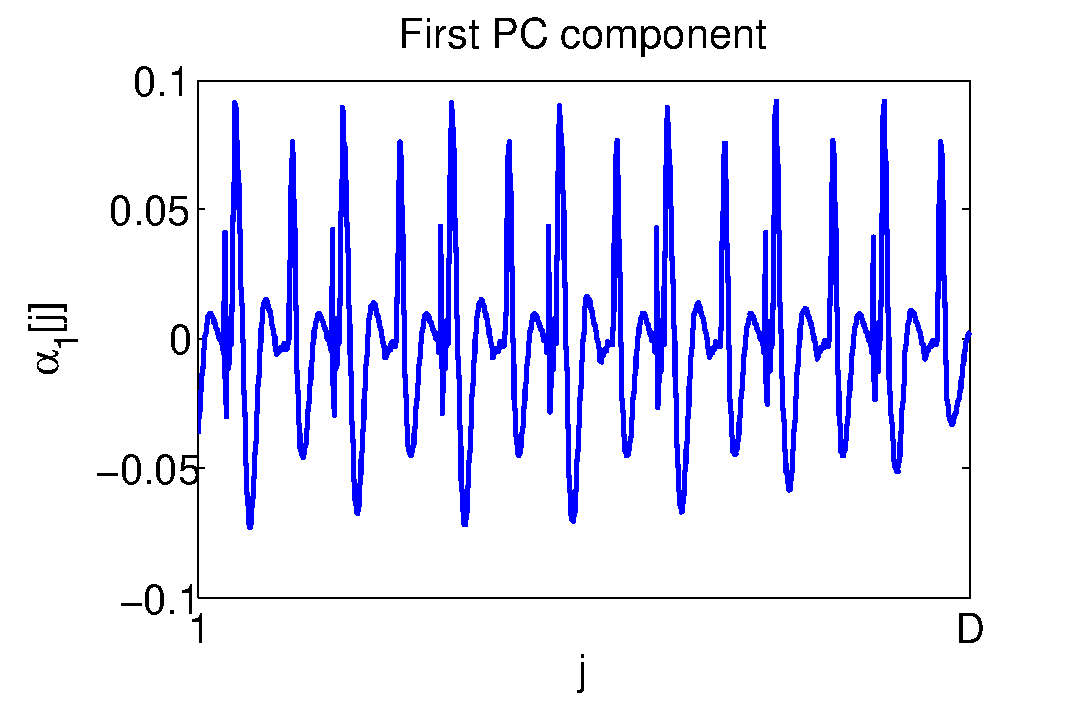
\includegraphics[width=.45\textwidth]{figures/DPAcontestPC1_new.pdf} 
%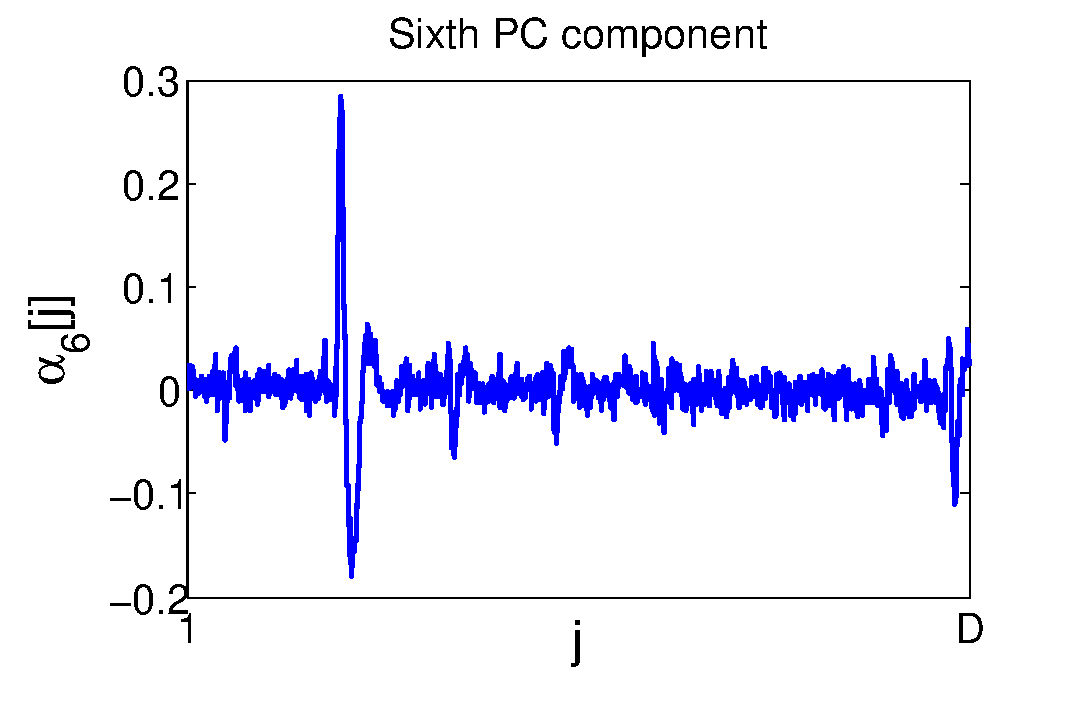
\includegraphics[width=.45\textwidth]{figures/DPAcontestPC6_new.pdf} 
%\caption{First and sixth PCs in DPA contest v4 trace set (between time samples 198001 and 199000)}\label{fig:DPAcontest}
%\end{figure}
%
Dans le contexte des impl�mentations s�curis�es, le but des d�veloppeurs est de minimiser les fuites, autrement dit, de r�duire le nombre de points de fuite, d'o� l'assomption suivante qui peut �tre raisonnablement faite: 

\begin{assumption}\label{assum:local}
L'information compromettante d'une trace acquis de canaux auxiliaires est localis�e en peu de points. 
\end{assumption}
Sous cette assomption, les auteurs de \cite{SCAclassProbl} ont donn� donn�e une deuxi�me r�ponse au probl�me du choix des composantes: ils utilisent le \emph{ratio de participation invers�} (IPR) pour �valuer la \emph{localisation} des vecteurs propres. Le IPR est ainsi d�fini:
\begin{equation}
\mathrm{IPR}(\AAlpha_i) = \sum_{j=1}^\traceLength \AAlpha_i[j]^4 \mbox{ .}
\end{equation}
Les auteurs de \cite{SCAclassProbl} sugg�rent de s�lectionner les PCs en ordre inverse par rapport �  leur IPR. \\

%
\subsubsection{La m�thode par variance expliqu�e locale} 
\begin{figure}
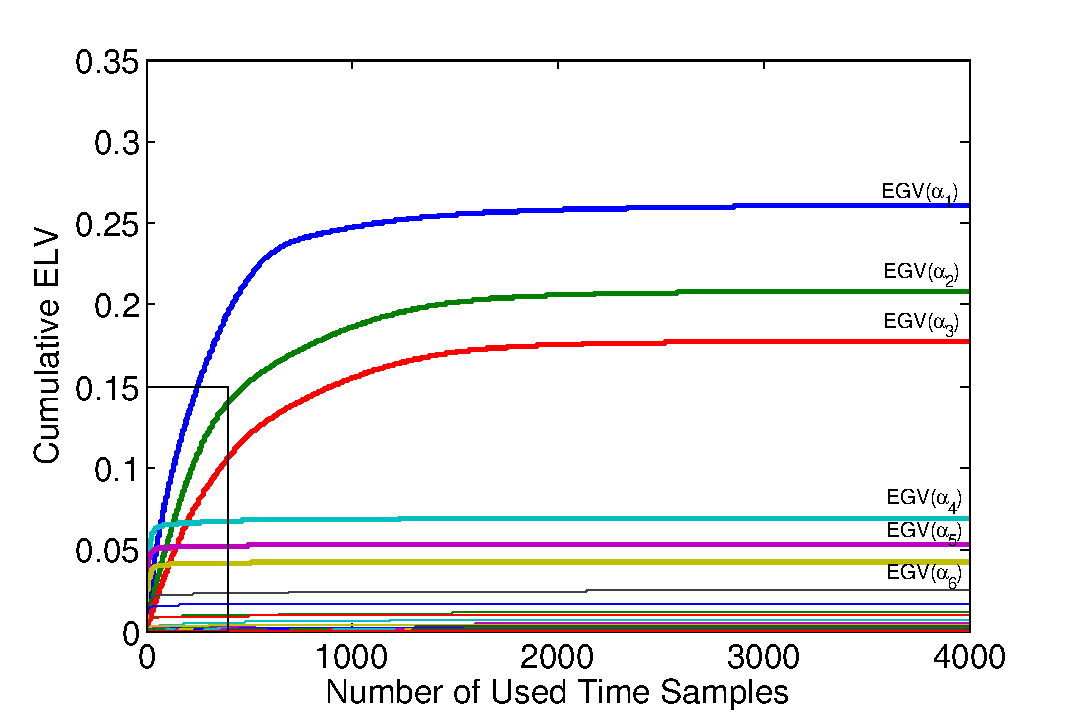
\includegraphics[width=0.5\textwidth]{figures/cumulativeELVallRectangle.pdf} 
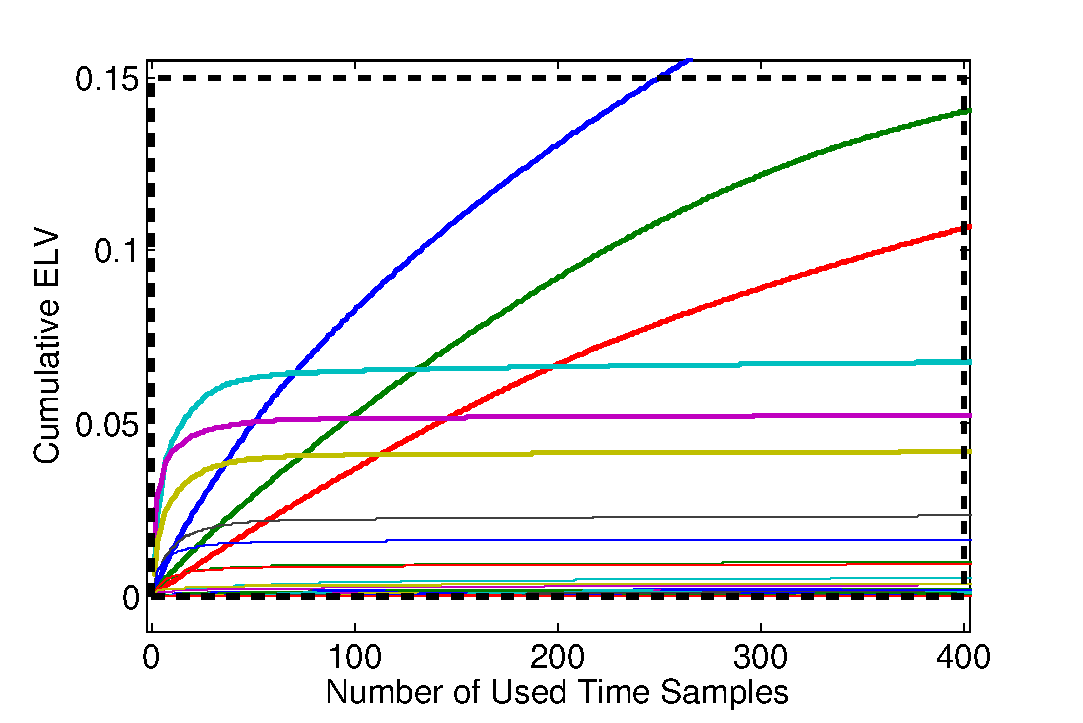
\includegraphics[width=0.5\textwidth]{figures/cumulativeELVzoomedRectangle.pdf} 
\caption{Cumulative ELV trend of principal components. On the right a zoom of the plot on the left. Acquisition campaign on an 8-bit AVR Atmega328P.}\label{fig:ELVcumulative}
\end{figure}
%
Les m�thodes de s�lection par EGV et IPR sont d'une certaine fa�on compl�mentaires : la premi�re se base uniquement sur les valeurs propres associ�es aux PC et ne consid�re pas la forme des PC elles-m�mes; la seconde ne consid�re pas l'information donn�e pas le valeurs propres, mais seulement la distribution des coefficients des PCs. Dans ce panorama nous avons propos� une nouvelle m�thode se s�lection qui fait un pont entre la EGV et la IPR : nous avons introduit la \emph{variance expliqu�e locale} (ELV) d'une PC $\AAlpha_i$ en un point $j$, d�finie par:
\begin{equation}
\mathrm{ELV}(\AAlpha_i,j) = \frac{\lambda_i \AAlpha_i[j]^2}{\sum_{k=1}^r\lambda_k} = \mathrm{EGV}(\AAlpha_i) \AAlpha_i[j]^2  \mbox{ .}
\end{equation}
Soit $\mathcal{J}=\{j^i_1, j^i_2, \dots, j^i_{\traceLength}\}\subset\{1,2,\dots,\traceLength\}$  un ensemble  d'indices ordonn�s de tel sort que $\mathrm{ELV}(\AAlpha_i,j^i_1)\geq \mathrm{ELV}(\AAlpha_i,j^i_2)\geq \dots \geq \mathrm{ELV}(\AAlpha_i,j^i_\traceLength)$. On observe que la somme sur tous les $\mathrm{ELV}(\AAlpha_i,j)$, pour tout $j\in[1,\dots,\traceLength],$  est �gal �  $\mathrm{EGV}(\AAlpha_i)$. Si on op�re cette somme en mani�re cumulative en suivant l'ordre donn�e par l'ensemble ordonn� $\mathcal{J}$, on obtient une description compl�te de la tendance suivie par la composante $\AAlpha_i$ pour atteindre son EGV. Comme montr� in Fig.~\ref{fig:ELVcumulative}, o� ces ELV cumulatives sont repr�sent�es, les trois premi�res composantes atteignent leur EGV finale tr�s lentement, alors que la $4$�me, $5$�me et $6$�me atteignent une large partie de leur EGV tr�s rapidement, c'est-� -dire an sommant les contributions ELV d'une moindre nombre de points. La s�lection par ELV, en analogie avec EGV, demande de fixer une taille pour la dimension r�duite du signal $\newTraceLength$, ou une seuil $\beta$ pour la ELV cumulative. Dans le premier cas les valeurs maximales de ELV de chaque PC sont compar�es, et les $\newTraceLength$ montantes les valeurs plus �lev�es sont s�lectionn�es. Dans le second cas, tous les couple (PC, point temporel) sont ordonn�s en ordre d�croissant de ELV, et somm�s jusqu'�  atteindre le seuil $\beta$. Les PC qui contribuent �  la somme sont s�lectionn�es.\\




\subsubsection{LDA et le probl\`{e}me du petit �chantillonnage}
L'extracteur $\extract^{\mathrm{LDA}}$ est une r�duction de dimension optimale, sous certaines conditions, pour r�soudre un probl�me de classification, c'est-� -dire un probl�me d'apprentissage o� l'on vise �  assigner �  une donn�e (une trace dans notre cas) un label (donn� ici par la valeur de la variable $\sensRandVar$ manipul�e lors de l'acquisition). Il a pour but non seulement d'�carter les centro\"ides par classe, mais aussi de reprocher au mieux les donn�es appartenant �  une m�me classe. La forte analogie entre les SCA et la t�che de classification en apprentissage automatique rend la LDA beaucoup plus adapt�e de la PCA dans ce contexte, mais plus co�teux. Comme la PCA, la LDA construit une matrice de projection $\textbf{A}$ en juxtaposant des vecteurs propres, les composantes lin�aires discriminantes (LDC), qui sont ceux de la matrice $\SW^{-1} \SB$, o� $\SB$ est d�finie en \eqref{eq:SB} et $\SW$ est la matrice des \emph{�carts intra-classe}:

\begin{equation}
\SW = \sum_{\sensVarGenValue\in\sensVarSet}\sum_{i=1\colon \sensVar_i=\sensVarGenValue}(\vLeakVec_i-\mmmXclass)(\vLeakVec_i-\mmmXclass)^\intercal \mbox{.}
\end{equation}

Le d�savantage principal de la LDA est appel� le \emph{probl�me du petit �chantillonnage} et se r�alise quand le nombre des traces $\nbTraces$ est inf�rieur ou �gal � leur taille $\traceLength$. Ceci implique que la matrice $\SW$ n'est pas inversible. Si la LDA a �t� introduite relativement r�cemment dans la litt�rature SCA, la communaut� de reconnaissance de patterns et apprentissage automatique cherche une solution � ce probl�me depuis les premi�res ann�es quatre-vingt-dix. Nous avons explor� les solutions propos�es, et les avons test�s sur des traces compromettantes. 

%
\subsubsection{R�sultats et conclusions}
\begin{figure}[t]
\subfigure[]{\label{fig:1.1}
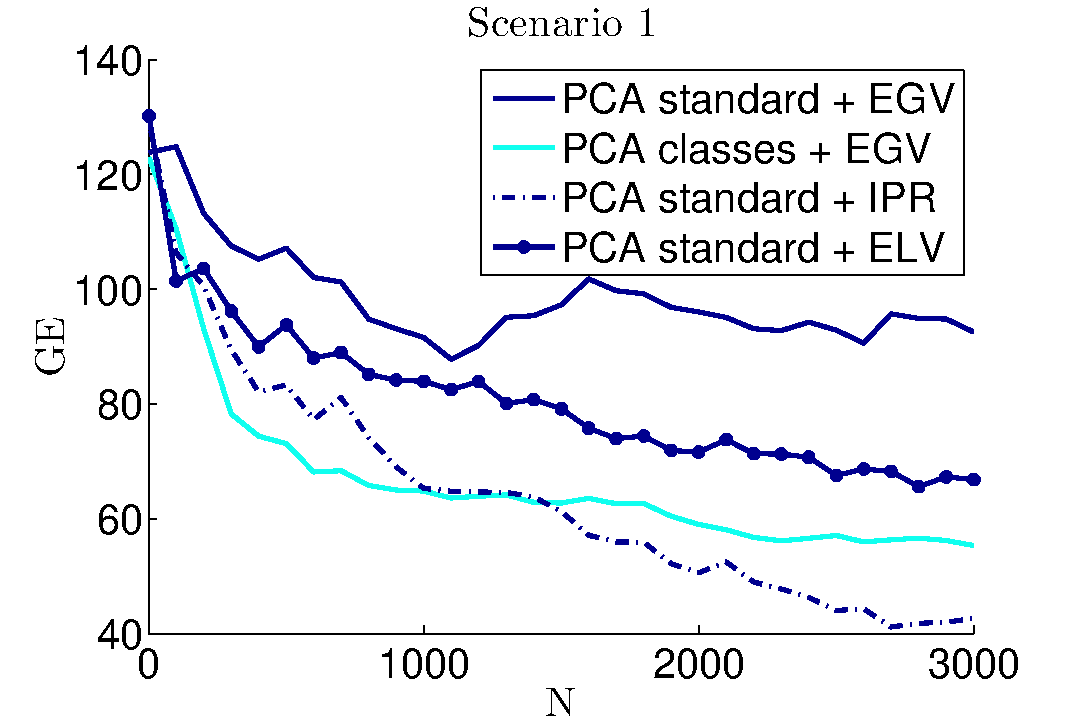
\includegraphics[width=0.5\textwidth]{figures/Criterion1.pdf}}
\subfigure[]{\label{fig:1.2}
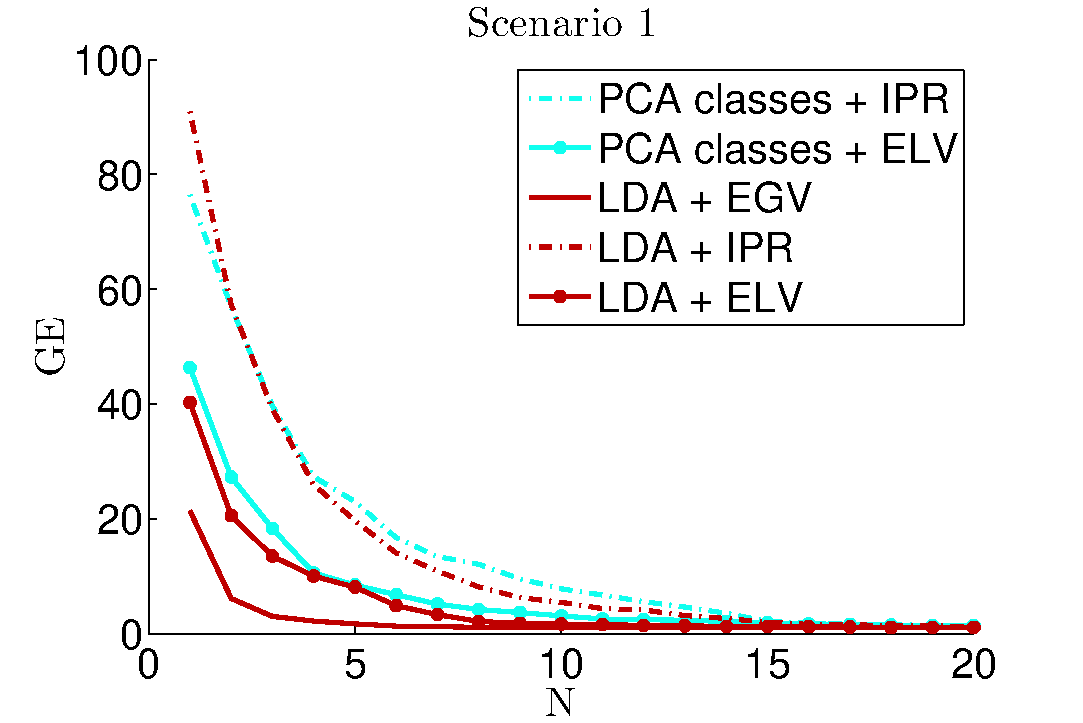
\includegraphics[width=0.5\textwidth]{figures/Criterion1Good.pdf}}
\caption{Guessing Entropy (rang moyen de la bonne hypoth�se de cl�) en fonction du nombre de traces d'attaque, pour diff�rentes m�thodes d'extraction. Les valeurs sont estim�es en moyennant le rang sur 100  exp�riences ind�pendantes.}\label{fig:scenario1}
\end{figure}

\begin{figure}
\subfigure[]{\label{fig:direct_PCA}
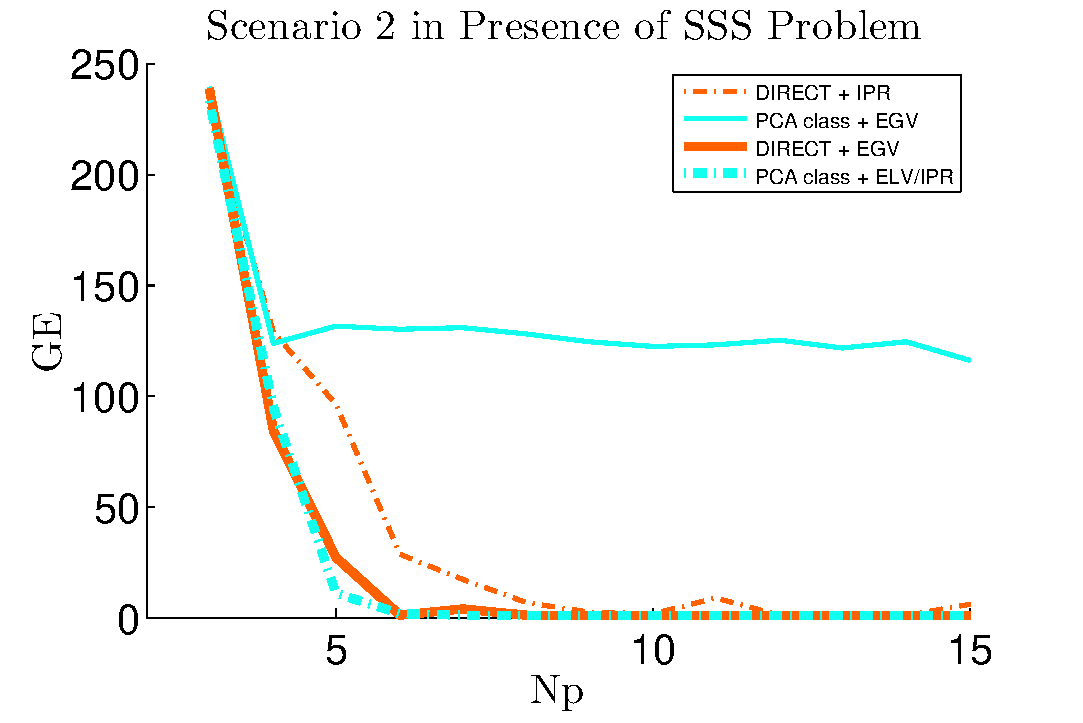
\includegraphics[width=0.5\textwidth]{figures/SSS.pdf}}
\subfigure[]{\label{fig:notSSS}
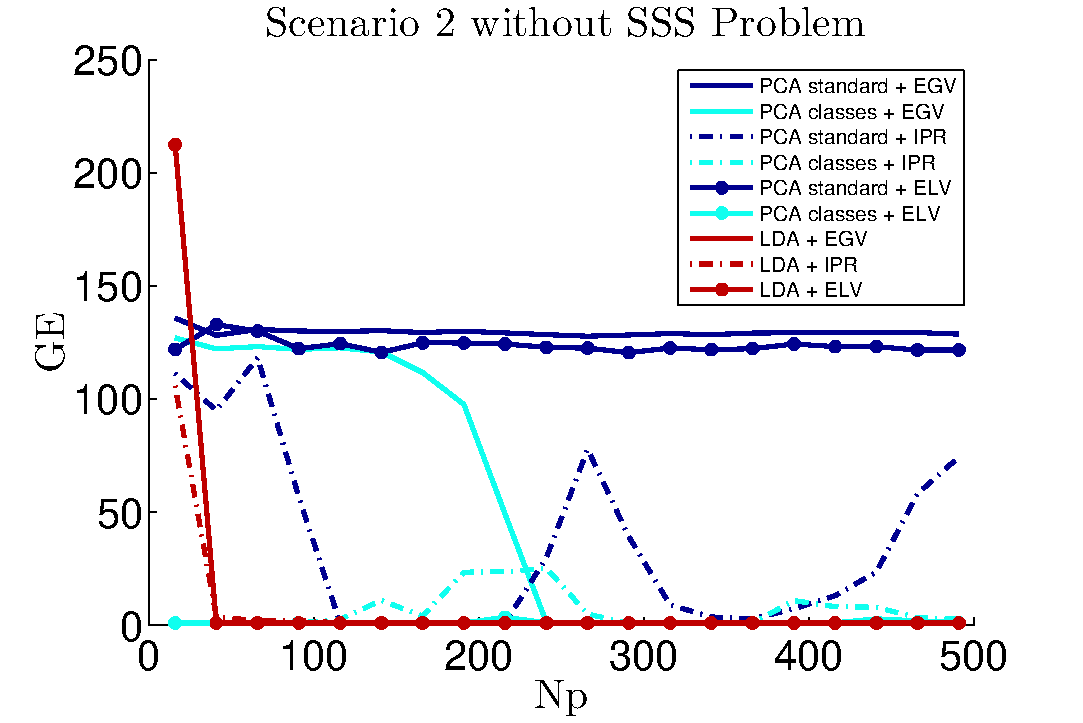
\includegraphics[width=0.5\textwidth]{figures/Criterion2notSSS.pdf}}
\caption{Guessing Entropy en fonction du nombre de traces de profilage. Figure \subref{fig:direct_PCA}: la meilleure extension de LDA et la PCA par profilage en pr�sence du probl�me du petit �chantillonnage; Figure \subref{fig:notSSS}: une comparaison en absence de probl�me du petit �chantillonnage.}\label{fig:scenario2}
\end{figure}

Nous avons men� diverses analyses exp�rimentales pour �valuer la m�thode de s�lection de composantes par ELV et les techniques d'extension de la LDA en pr�sence du petit �chantillonnage. Dans cette section nous reportons les plus significatifs, en les extrayant du chapitre 4 de la th�se. Nous consid�rons ici deux sc�narios: dans le premier (Scenario 1) l'attaquant a un large nombre de trace de profilage ($\nbProfilingTraces$) et veut minimiser le nombre de traces d'attaque ($nbAttackTraces$) pour obtenir une attaque r�ussie. En observant la Fig.~\ref{fig:scenario1} nous pouvons tirer trois conclusions: 
\begin{itemize}
\item nous confirmons que la PCA standard est bien sous-optimale par rapport � la PCA par profilage
\item nous confirmons que la LDA est plus adapt�e de la PCA pour pr�-traiter le traces par canaux auxiliaires
\item en �quipant la PCA profil�e avec la m�thode de s�lection par ELV (� la place de la EGV classique) les performances de l'attaque augmentent significativement, en se rapprochant de celles obtenues � travers la LDA.
\end{itemize}
Dans le Scenario 2, l'attaquant veut au contraire minimiser le nombre de traces de profilage n�cessaires pour obtenir une bonne m�thode de pr�-traitement et profilage. Dans ce cas, le probl�me du petit �chantillonnage peut se v�rifier. En observant la Fig.~\ref{fig:scenario2} nous concluons que encore une fois, en pr�sence ou pas du petite �chantillonnage, la PCA �quip� de la s�lection par ELV a performances proches de celles de la LDA ou de sa meilleure alternative en pr�sence du petit �chantillonnage.


\subsection{Analyse Discriminante par Noyau}\label{sec:kda}
Quand une contre-mesure de masquage d'ordre $(d-1)$ est mise en place, la targette $\sensRandVar$ est repr�sent�e par une $d$-uple de partie $M_i$ manipul�es � diff�rents instants temporels $t_1,\dots,t_d$ et l'information sensible r�side dans le moment $\esper[\vaLeakVec[t_1]\vaLeakVec[t_2]\cdots \vaLeakVec[t_d]]$ d'ordre $d$, c'est-�-dire que la fonction  $f(z) = \esper[\vaLeakVec[t_1]\vaLeakVec[t_2]\cdots \vaLeakVec[t_d]\vert Z=z]$ n'est pas constante. Pour exploiter cette information cela a �t� montr�  \cite{carlet2014achieving} qu'il est n�cessaire de consid�rer une statistique des donn�e qui, vu comme polyn�me multivari� dans les coordonn�es de $\vaLeakVec$, contient le mon�me de degr� $d$ $\prod_{i=1,\dots,d}\vaLeakVec[t_i]$. Comme en pratique les points $t_1,\dots,t_d$ sont inconnus � l'attaquant, une id�e na�ve pour obtenir un extracteur effectif et de chercher parmi les combinaisons lin�aires des produits de tous les possibles $d$-uples de points. Ceci revient � immerger les donn�es � travers une fonction non-lin�aire $\Phi$ dans un espace de grand dimension $\featureSpace = \mathbb{R}^{D\choose{d}}$, et ici appliquer les m�thodes d'extraction lin�aires (LDA et PCA, par exemple). L'espace $\featureSpace$ est appel� dans \emph{espace des caract�ristiques}, car c'est l'espace qui contient les caract�ristiques informatives des traces. La croissance combinatoire de la taille de $\featureSpace$ est un obstacle d'un point de vu calculatoire, car ce demande de manipuler et stocker des traces de taille ${D\choose{d}}$. L'algorithme KDA permet � un attaquant d'utiliser l'extracteur LDA dans $\featureSpace$  sans effectuer de calculs dans l'espace $\featureSpace$, comme sch�matis� dans la Fig.~\ref{fig:scheme2}.\\

L'outil central de l'astuce du noyau est la \emph{fonction noyau} $K \colon \mathbb{R}^\traceLength \times \mathbb{R}^\traceLength \rightarrow \mathbb{R}$, qui doit satisfaire la propri�t� suivante, en r�lation avec la fonction $\Phi$:

\begin{equation}\label{eq:kernelProperty}
K(\vLeakVec,\yyy) = \Phi(\vLeakVec)\cdot \Phi(\yyy) \mbox{ ,}
\end{equation}
pour toute donn�e $\vLeakVec$ et $\yyy$, o� $\cdot$ est le produit scalaire.

Toute fonction $\Phi$ a une fonction noyau associ�e, donn�e \eqref{eq:kernelProperty}, pour un ensemble de donn�es. Au contraire, seulement les fonctions $K\colon\mathbb{R}^D\times \mathbb{R}^D \rightarrow \mathbb{R}$ qui satisfont une condition de convergence connue comme {\em condition de Mercer} sont associ�es � une map $\Phi:\mathbb{R}^D \rightarrow \mathbb{R}^F$, pour quelque $F$. Les fonctions noyau �ligibles pour une astuce du noyau sont celles qui sont calculables directement � partir des donn�es brutes $\vLeakVec_i$, sans �valuer la fonction $\Phi$. \\
%
%The notion of kernel function is illustrated in the following example.
%
%\begin{example}\label{ex:polyKernel}
%Let $D=2$. Consider the function
%\begin{align}
%&K\colon\mathbb{R}^2\times \mathbb{R}^2 \rightarrow \mathbb{R} \nonumber \\ 
%&K\colon(\sss[]{i},\sss[]{j}) \mapsto ( \sss[]{i}\cdot \sss[]{j})^2 \mbox{ ,} \label{eq:example1}
%\end{align}
%
%After defining $\sss[]{i} = [a,b]$ and $\sss[]{j} = [c,d]$, we get the following development of K:
%\begin{equation}
%K(\sss[]{i},\sss[]{j}) = (ac + bd)^2 = a^2c^2 + 2abcd + b^2d^2 \mbox{ ,}
%\end{equation}
%
%which is associated to the following map from $\Bbb{R}^2$ to $\Bbb{R}^3$:
%
%\begin{equation}
%\Phi(u,v) =  [u^2, \sqrt{2}uv, v^2]
%\end{equation}
%
%Indeed $\Phi(\sss[]{i})\cdot \Phi(\sss[]{j}) = a^2c^2 + 2abcd + b^2d^2 = K(\sss[]{i},\sss[]{j})$\enspace. This means that to compute the dot product between some data mapped into the $3$-dimensional space $\featureSpace$ there is no need to apply $\Phi$: applying $K$ over the $2$-dimensional space is equivalent. 
%
%\end{example}
%
%
\begin{figure}
\centering
{
\begin{tikzpicture}
\matrix (m) [matrix of math nodes, row sep=3em,
column sep=3em, text height=1.5ex, text depth=0.25ex]
{ \mathbb{R}^\traceLength & \featureSpace & \mathbb{R}^\newTraceLength \\};
\path[->]
(m-1-1) edge node[above] {$\Phi$} (m-1-2);
         %edge [bend left=30] (m-2-2)
         %edge [bend right=15] (m-2-2);
\path[->]
($(m-1-2.north east)-(0,0.1)$) edge node[above] {$\extract^{\mathrm{PCA}}$} ($(m-1-3.north west)-(0,0.1)$);
\path[->]
($(m-1-2.south east)+(0,0.15)$) edge node[below] {$\extract^{\mathrm{LDA}}$} ($(m-1-3.south west)+(0,0.15)$);

\path[->]
(m-1-1) edge [bend left=50] node[above] {$\extract^{\mathrm{KPCA}}$} (m-1-3)
(m-1-1) edge [bend right=50] node[below] {$\extract^{\mathrm{KDA}}$} (m-1-3);

\end{tikzpicture} 
}
\caption{Applying KDA and KPCA permits to by-pass computations in $\featureSpace$.}\label{fig:scheme2}
\end{figure}
%
La fonction noyau \emph{polynomiale de degr� $d$} fait partie de ce type de fonctions. Elle est ainsi d�finie: 
\begin{equation}
K(\vLeakVec_i,\vLeakVec_i) = (\vLeakVec_i \cdot \vLeakVec_j)^d \mbox{ ,}
\end{equation}
et corresponde � la fonction $\Phi$ qui porte les coordonn�es en entr�e dans l'espace des caract�ristiques qui contient tous les possibles mon�mes de degr� $d$ dans ces coordonn�es, � constants pr�s. Elle est donc, � constants pr�s, la fonction $\Phi$ du sch�ma de Fig.~\ref{fig:scheme2}. L'algorithme pour obtenir $\extract^\mathrm{KDA}$ est le suivant.
%
\subsubsection*{KDA pour traces masqu�es � l'ordre $d$}\label{procedure:KDA}
�tant donn� un ensemble de traces de profilage $(\vLeakVec{i},\sensVar_i)_{i=1,\dots, \nbTrainingTraces}$ et la fonction noyau $K(\vLeakVec,\yyy)= (\vLeakVec\cdot \yyy)^d$:
\begin{itemize}
\item[1)] Construire une matrice $\MMM$ (elle agit comme \emph{matrice des �carts inter-classe}):

\begin{equation}
\MMM = \sum_{\sensVarGenValue\in\sensVarSet}\nbTracesPerClass(\MMMclass - \MMMT)(\MMMclass-\MMMT)^\intercal\mbox{ ,}
\end{equation}

o� $\MMMclass$ et $\MMMT$ sont deux vecteurs colonne de taille $N$, avec coordonn�es donn�es par:
\begin{align}
\MMMclass[\sensVarGenValue][j] = \frac{1}{\nbTracesPerClass}\sum_{i:\sensVar_i=\sensVarGenValue}K(\vLeakVec_j,\vLeakVec_i)\\
\MMMT[j] = \frac{1}{\nbTrainingTraces}\sum_{i=1}^{\nbTrainingTraces}K(\vLeakVec_{j},\vLeakVec_{i}) \mbox{ .}
\end{align}

\item[2)] Construire une matrice $\NNN$ (elle agit comme \emph{matrice des �carts intra-classe}):
\begin{equation}\label{eq:N}
\NNN = \sum_{\sensVarGenValue\in\sensVarSet}\kernelMatrix_\sensVarGenValue(\III - \III_{\nbTracesPerClass})\kernelMatrix_\sensVarGenValue^\intercal\mbox{ ,}
\end{equation}
o� $\III$ est la matrice identit� de taille $\nbTracesPerClass \times \nbTracesPerClass$, $\III_{\nbTracesPerClass}$ est la matrice de taille $\nbTracesPerClass \times \nbTracesPerClass$ avec tous les �l�ments �gals � $\frac{1}{\nbTracesPerClass}$ et $\kernelMatrix_{\sensVarGenValue}$ est la sous-matrice de $\kernelMatrix = (K(\vLeakVec_i,\vLeakVec_j))_{\substack{i=1,\dots,\nbTrainingTraces \\ j=1,\dots,\nbTrainingTraces}}$ de taille $\nbTrainingTraces \times \nbTracesPerClass$ qui contients toutes les colonnes index�es par les $i$ tels que $\sensVar_i=\sensVarGenValue$. 

\item[3)] R�gulariser la matrice $\NNN$ pour garantir la stabilit� calculatoire et g�rer le \emph{surapprentissage}:
\begin{equation}\label{eq:mu}
\NNN = \NNN + \mu  \III
\end{equation}

\item[4)] Trouver les valeurs propres non nulles $\lambda_1, \dots, \lambda_\numEigenvectors$  de $\NNN^{-1}\MMM$ et le vecteurs propres correspondant $\nununu_1, \dots, \nununu_\numEigenvectors$; 


\item[5)] Finalement, la projection d'une nouvelle trace $\vLeakVec$ sur la $\ell$-i�me composante discriminante d'ordre $d$ se calcule ainsi:
\begin{equation}\label{eq:projectionKDA}
\extract^{\mathrm{KDA}}_{\ell}(\vLeakVec) = \sum_{i=1}^{\nbTrainingTraces}{\nununu}_\ell[i]K(\vLeakVec_i, \vLeakVec) \mbox{ .}
\end{equation} 

\end{itemize}

\subsubsection{Analyse and r�sultats}
\begin{figure}[t]
\subfigure[]{\label{fig:numClasses-2order}
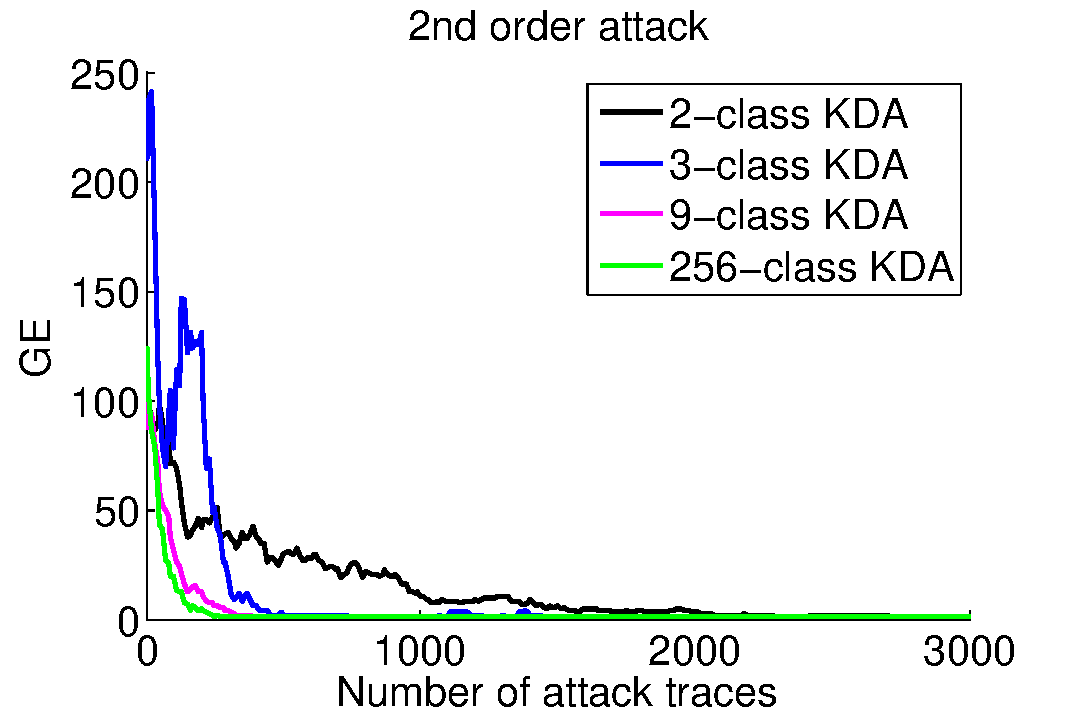
\includegraphics[width=.5\textwidth]{figures/2order_classes_TA.pdf}}
\subfigure[]{\label{fig:numClasses-3order}
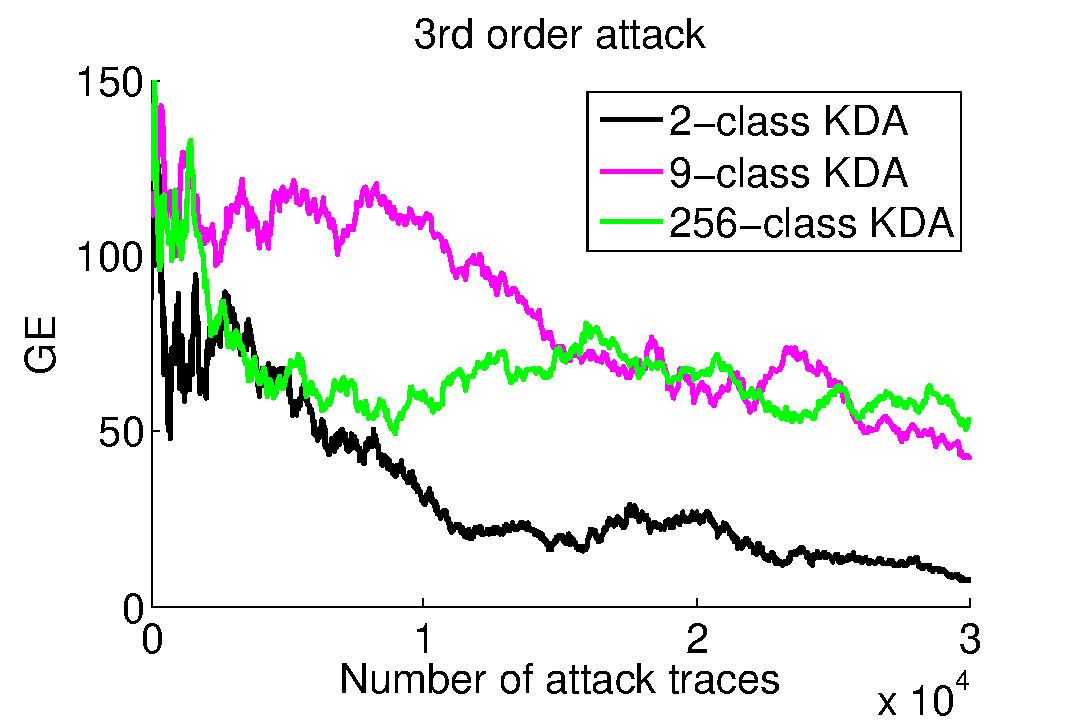
\includegraphics[width=.5\textwidth]{figures/3order_new.pdf}}
\caption{Comparaison entre KDA sous 2 classes, 3 classes, 9 classes and 256 classes KDA dans un contexte d'attaque de $2$nd ordre \subref{fig:numClasses-2order} et de $3$�me ordre \subref{fig:numClasses-3order}. Pour le $2$nd ordre, la KDA est efficace � dissocier les donn�es en 256 classes, permettant une caract�risation optimale. Pour le $3$�me ordre les donn�es de profilage ne sont pas en nombre suffisant pour r�ussir une phase de caract�risation en 256 classes distingu�es. Diminuer le nombre de classes � dissocier, fait am�liorer l'efficacit� du pr�-traitement et, en cons�quence, de l'attaque. }\label{fig:numClasses}
\end{figure}

Le premier aspect de l'application de la KDA sur lequel nous nous sommes concentr� est l'importance d'une bonne r�gularisation (obtenue par le choix du param�tre$\mu$ in \eqref{eq:N}) : cette r�gularisation est la r�ponse au fait que les m�thodes par noyau sont souvent port� au surapprentissage: ceci signifie, dans le cas de la KDA, que $\extract^{\mathrm{KDA}}$ risque de grouper parfaitement les traces d'apprentissage dans leur classe, mais de ne pas r�ussir � dissocier les traces d'attaque. La r�gularisation consiste � rajouter une contrainte � la phase d'apprentissage, dans le but de cr�er un mod�le qui ait le plus possible le m�me comportement avec les traces d'apprentissage et les nouvelles donn�es sur lequel s'applique. Nous avons observ� que le extracteurs issus d'une bonne r�gularisation tiraient leurs projections de zones des traces tr�s localis�es, ce qui est encore signe (comme pour les extracteurs lin�aires) d'une bonne d�tection implicite des PoIs. 

%
Le deuxi�me aspect sur lequel nous nous sommes concentr� est le r�le de la forme de la targette dans le compromis pr�cision-efficacit�. Du fait que la complexit� calculatoire de la KDA est $O(\nbTrainingTraces^3)$, avec $\nbTrainingTraces$ est le nombre des traces d'apprentissage,  il peut �tre int�ressant de diminuer ce nombre $\nbTrainingTraces$ pour augmenter l'efficacit� du calcul. Cependant, borner $\nbTrainingTraces$ r�duit la pr�cision de la KDA. Une mani�re de pallier � cette perte de pr�cision est de r�duire le nombre de classes � dissocier, en choisissant comme targette une fonction non-injective d'une variable interne du calcul cryptographique $m(\sensRandVar)$. Par example, les valeurs de $\sensRandVar$ peuvent �tre group�s selon leur poids d'Hamming: un mod�le � 2 classes est donn� par ($m(z) =0$ if $\HW(z)<4$, $m(z) =1$ if $\HW(z)\geq4$). Une fois r�alis� un pr�-traitement bas� sur un certain mod�le non-injectif, il parait ad�quat r�aliser l'attaque en visant la m�me targette. Ayant fix� le nombre $\nbTrainingTraces$ pour les traces d'apprentissage, les r�sultats de ce type d'attaque sont montr�s en Fig.~\ref{fig:numClasses} : si dans un contexte d'attaque de $2$nd ordre, on peut observer que la KDA s'entra�ne sur un nombre suffisant de donn�es pour r�ussir une s�paration en 256 classes, pour des contextes d'ordre sup�rieur la conversion � un probl�me � 2 classes devient une meilleure strat�gie.

\begin{figure}
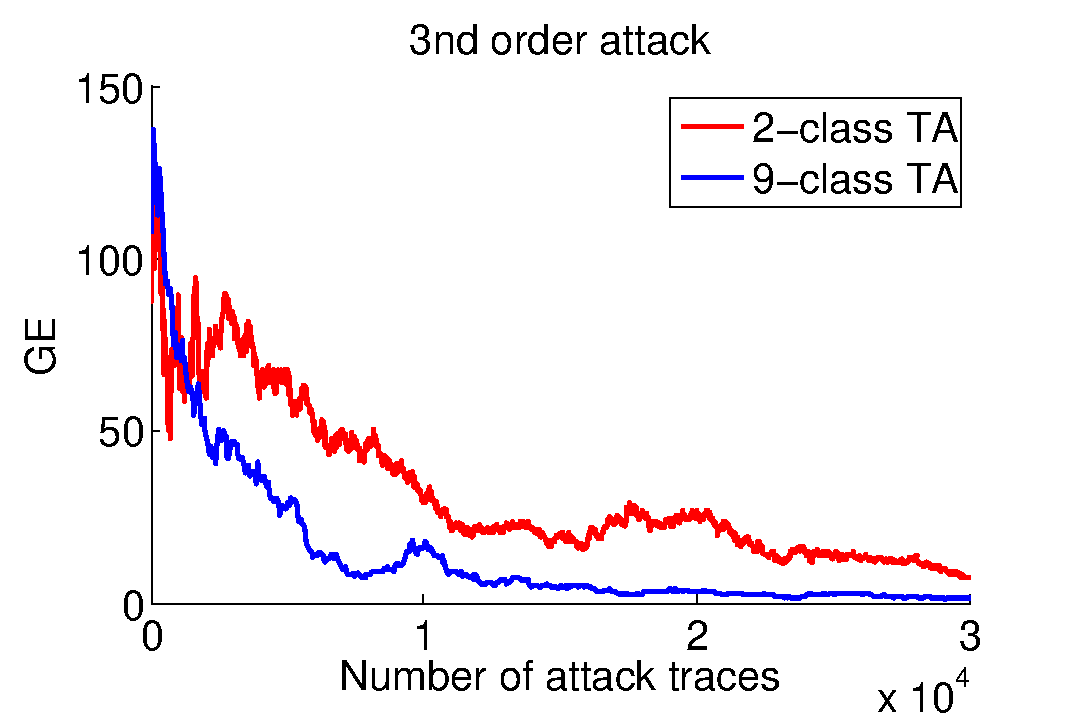
\includegraphics[width=.5\textwidth]{figures/3order_2_9.pdf} 
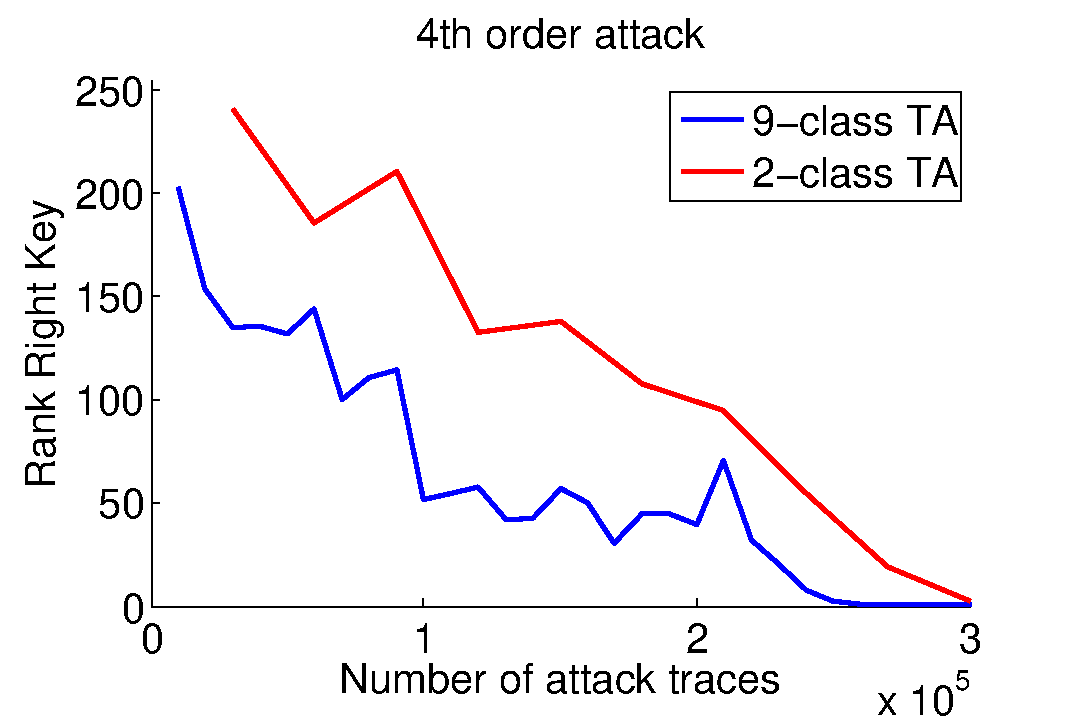
\includegraphics[width=.5\textwidth]{figures/4order_2_9.pdf} 
\caption{Gauche: guessing entropy  pour des attaques \emph{template} d'ordre 3, � 2 classes et � 3 classes. Droite: rang de la bonne cl� pour une attaque d'ordre 4 � 2 classes et � 9 classes.}\label{fig:3-4}
\end{figure}

%Third, I evaluated the soundness of an asymmetric preprocessing-attack approach. The success of a 2-class extractor always relies on a good exploitation of the PoIs, whose position does not depend on the chosen target model. For this reason, even if an extractor has been trained to separate $W$ classes, it does not mean that a finest characterization is useless. Results depicted in Fig.~\ref{fig:3-4} come from this asymmetric approach: the extractors used have been trained over $2$ classes, but the attacks that exploit a $9$-class characterization are more efficient.  
%
%Finally, I effectuated a comparison between the KDA and the PP approach. In particular I compared their performances under a fixed training set size, concluding that the effectiveness of the KDA is much less affected by the increase of the order $d$ than the PP. Indeed, the latter failed the PoI detection at orders 3 and 4.


\subsection{R�seaux Neuronaux Convolutifs}\label{sec:cnn}
Dans cette derni�re partie, nous adoptons une strat�gie d'attaque bas�e sur le paradigme de l'apprentissage profond: � l'aide de r�seaux neuronaux � plusieurs couches nous ne s�parons plus la routine d'apprentissage en pr�-traitement et caract�risation, mais int�grions les pr�-traitement de fa�on implicite dans l'apprentissage. Les r�seaux neuronaux, gr�ce � leurs architectures facilement parall�lisables, sont les outils privil�gi�s aujourd'hui pour r�soudre le probl�me de la classification sur des donn�es de grandes dimension, comme les signaux compromettants. Nous nous int�ressons en particulier aux r�seaux neuronaux convolutifs (\emph{Convolutional Neural Networks}, en anglais, CNN): �tant con�us pour �tre robustes aux d�formations g�om�triques des donn�es, typiques dans le contexte de la reconnaissance de l'image, ils nous ouvrent une nouvelle strat�gie pour faire face aux contremesures bas�es sur l'augmentation de la d�synchronisation dans les acquisitions. Nous nous pla�ons donc dans ce contexte, en menant des exp�riences d'attaque contre ce type de contremesures, en utilisant un r�seau CNN, et en �quipant la routine d'apprentissage de strat�gies d'augmentation des donn�es (\emph{Data Augmentation}, DA) d�sign�es pour le contexte des signaux d�synchronis�s. Apr�s une br�ve introduction de ces outils, nous reportons les r�sultats des exp�riences en Sec.~\ref{sec:cnn_res}.

\subsubsection{Architecture et apprentissage}
Les CNNs appartiennent � la famille plus r�pandue de r�seaux neuronales est celle des \emph{Multi-Layer Perceptrons} (MLP). On peut exprimer un MLP destin� � la classification dans la forme:
\begin{equation}\label{eq:MLP}
\MLmodel(\vLeakVec) = \softmax\circ\lambda_n\circ\sigma_{n-1}\circ\lambda_{n-1}\circ\dots\circ \lambda_1(\vLeakVec)=\yyy \mbox{ ,}
\end{equation}
o�:
\begin{itemize}
\item Les fonctions $\lambda_i$ sont appel�es couches enti�rement connect�es (\emph{Fully-Connected},FC) et s'expriment comme fonctions affines $\textbf{A}\vLeakVec + \vec{b}$, avec $\textbf{A}\in\mathbb{R}^{D\times C}$ une matrice de poids et $\vec{b}\in\mathbb{R}^C$ un vecteur de biais, � optimiser � travers l'apprentissage. Ces couches extraient lin�airement de l'information des donn�es, de la m�me mani�re que les techniques PCA ou LDA.

\item  Les fonctions $\sigma_i$ sont appel�es couches d'\emph{activation} (ACT): elles sont g�n�ralement non-lin�aires, s'appliquent souvent ind�pendamment � chaque coordonn�e de l'entr�e, et ne d�pendent pas de param�tres entrainables. 
 

\item $\softmax$ est la fonction \emph{softmax}:: $\softmax(\vLeakVec)[i] = \frac{e^{\vLeakVec[i]}}{\sum_{j}e^{\vLeakVec[j]}}$. Elle normalise la sortie du r�seaux en la rendant interpr�table comme distribution de probabilit� $\MLmodel(\vLeakVec) \approx \pdf_{\given{\sensRandVar}{\vaLeakVec=\vLeakVec}}$.
\end{itemize}
 
Les r�seaux convolutifs s'obtiennent en rajoutant aux MLPs deux autres typologies de couches:
\begin{itemize}
\item les couches convolutifs (CONV) $\gamma$, sont des couches lin�aires qui partagent leurs poids � travers l'espace. Elles extraient de l'information lin�airement � travers des filtres de poids qui agissent localement. Ces filtres glissent le long de leurs entr�e et leur action locale est r�p�t�e sur toute position de l'entr�e. Ceux sont les couches qui se chargent de rendre le r�seau robuste aux d�formations qui d�placeraient les informations le long de la traces, donc � la d�synchronisation.
\item Le couches de pooling (POOL) $\delta$ effectuent un sous-�chantillonnage des donn�es partielles trait�es par le r�seaux afin de r�duire la complexit� du calcul d�riv�e de l'extraction d'un nombre croissant de caract�ristiques, niveau par niveau, par les couches CONV.
\end{itemize}

Les param�tres d'un r�seau neuronal sont � entrainer pendant la phase d'apprentissage. La plus utilis�e des m�thodes d'optimisation est la \emph{descente de gradient stochastique}, qui est mise en place dans le but de minimiser un fonction de co�t qui quantifie l'erreur de classification du r�seau sur l'ensemble d'apprentissage. Elle consiste en:

\begin{itemize}
\item s�lectionner un  \emph{mini-lot} de traces d'apprentissage $(\vLeakVec_i, \sensVar_i)_{i\in I}$ choisies en ordre al�atoire (ici $I$ est un ensemble al�atoire d'indices)
\item calculer les outputs du mod�le courant pour le mini-lot s�lectionn� $(\vNNOutput_i = \MLmodel(\vLeakVec_i))_{i\in I}$, 
\item �valuer la fonction de co�t, dans le cas de nos exp�riences il s'agit de l'entropie crois�e:
\begin{equation}\label{eq:lossfunction}
\mathcal{L} = -\frac{1}{\lvert I \rvert} \sum_{i\in I} \sum_{t=1}^{|\sensVarSet|}\vec{\sensVar_i}[t]\log{\vNNOutput_i[t]} \mbox{ ,}
\end{equation} 
\item calculer les d�riv�es partielles de la fonction de co�t, par rapport aux param�tres entrainables, � l'aide de la m�thode de \emph{r�tropropagation du gradient},
\item mettre � jour les param�tres entrainables en soustrayant un petit multiple (appel�  \emph{taux d'apprentissage}) du gradient.
\end{itemize}  

Une it�ration compl�te sur l'ensemble d'apprentissage est appel�e \emph{�poque}.
Le la nature des couche, leur nombre et leurs tailles sont les hyper-param�tres qui d�finissent l'architecture d'un r�seaux. Le nombre d'�poques, la taille des mini-lots et le taux d'apprentissage, sont aussi des hyper-param�tres qui r�glent l'apprentissage. 


\subsubsection{Augmentation des Donn�es}\label{sec:DA}

\begin{figure}[t]
\centering
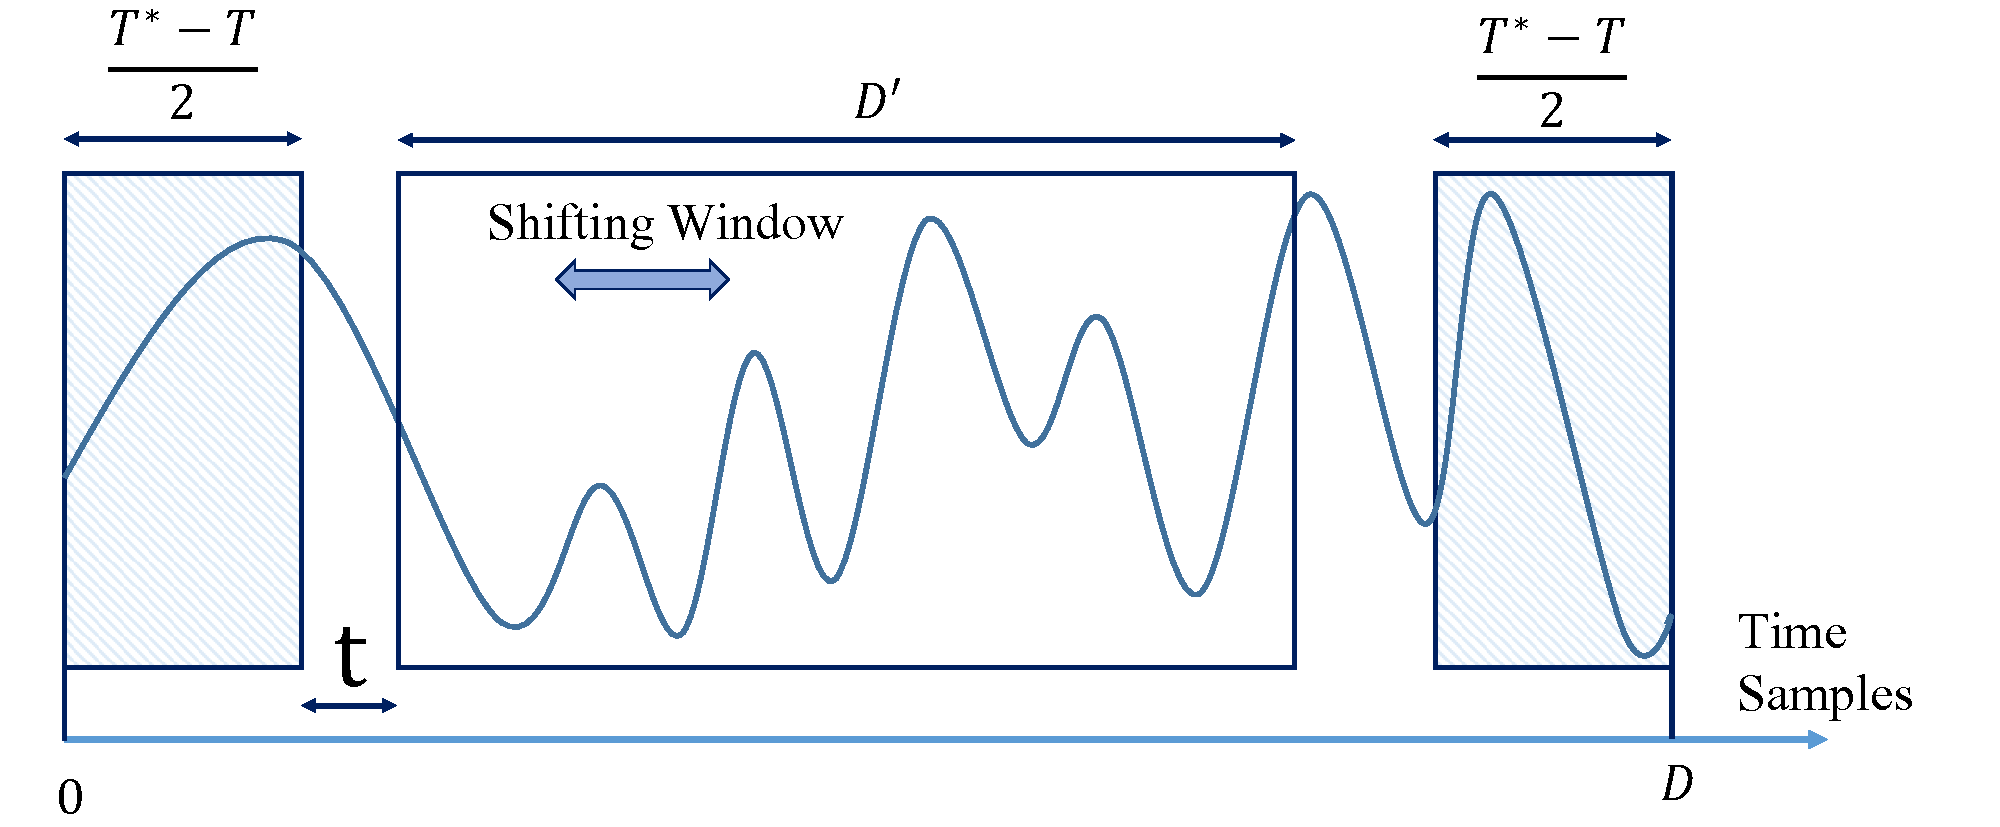
\includegraphics[width=.4\textwidth]{../Figures/CHES2017/Shifting_window.pdf}
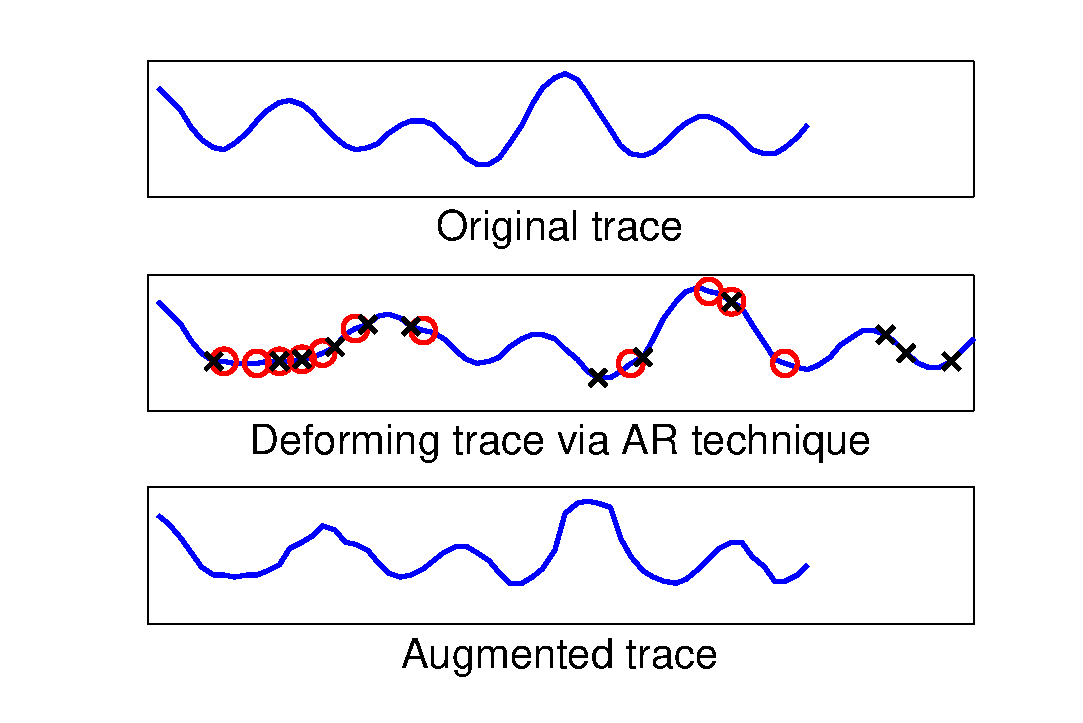
\includegraphics[width=.4\textwidth]{../Figures/CHES2017/AR_example.pdf}
\caption{Gauche: M�thode Shifting pour DA. Droite: M�thode Add-Remove pour DA (les points ajout�s sont marqu�s par des cercles rouges, les points supprim�s par des croix noires.}\label{fig:AR}
\end{figure}

Quand un r�seau neuronal a une grande capacit�, c'est-�-dire peut exprimer des mod�les tr�s complexes, et est entrainer avec un nombre insuffisant de donn�es, il risque de provoquer du surapprentissage. Une mani�re classique de r�duire ce probl�me est l'introduction des m�thodes d'augmentation des donn�es. Elles consistent � g�n�rer artificiellement des nouvelles donn�es d'apprentissage, en d�formant celles r�ellement acquises. La d�formation est obtenu en appliquant des d�formations qui pr�servent la targette de la classification, c'est-�-dire la valeur de la variable sensible manipul�e lors de l'acquisition. Nous avons propos�e deux techniques d'augmentation des donn�es appel�es \emph{Shifting} et \emph{Add-Remove}

\paragraph*{Shifting ($\mathrm{SH}_{T^\star}$)} Cette technique simule un effet de d�lai al�atoire d'amplitude maximale $T^\star$, en s�lection une fen�tre glissante d'une signal acquis, comme montr� en Fig. \ref{fig:AR}. Soit $\traceLength$ la taille originale du signal. Nous fixons la taille d'entr�e de la premi�re couche du r�seau neuronal �  $\traceLength^\prime = \traceLength - T^\star$. La technique $\mathrm{SH}_{T^\star}$ consiste alors (1) � tirer un al�a uniform $t \in[0,T^\star]$, et (2) � s�lectionner la fen�tre de taille $\traceLength^\prime$ � partir du $t$-�me point de la trace. Pour notre �tude, nous souhaitons comparer les techniques $\mathrm{SH}_T$ pour diff�rent valeurs de $T \leq T^\star$, sans changer l'architecture du r�seau utilis� (en particulier la taille de l'entr�e $\traceLength^\prime$). Notamment, $T \lneq T^\star$ implique que $T^\star-T$ points temporels ne sont certainement jamais s�lectionn�s. Comme nous supposons que l'information est localis�e dans la partie centrale de l'acquisition, nous choisissons de centrer les fen�tre glissantes, en supprimant les premiers et les derniers $\frac{T^\star-T}{2}$ points des traces. 

\paragraph*{Add-Remove ($\mathrm{AR}$)}  Cette technique simule un effet de jitter de l'horloge (Fig. \ref{fig:AR}). Nous d�notons par  $\mathrm{AR}_R$ l'op�ration qui consiste en deux �tapes:
\begin{itemize}
\item[(1)] ins�rer  $R$ points temporels, dont la position est choisi de fa�on al�atoire uniforme et dont la valeur est obtenue par moyenne arithm�tique entre le point qui suit et celui qui pr�c�de,
\item[(2)] supprimer $R$ points temporels, choisis de fa�on al�atoire uniforme.\\
\end{itemize}

Ces deux d�formations peuvent �tre compos�es: nous d�notons par $\mathrm{SH}_T\mathrm{AR}_R$ l'application de $\mathrm{SH}_T$ suivie par celle de $\mathrm{AR}_R$.
 

\subsubsection{R�sultats exp�rimentaux}\label{sec:cnn_res}
Pour les diverses exp�riences men�es nous avons r�gl� et fix� une fois pour toutes l'architecture de r�seau convolutif utilis�e:
\begin{equation}\label{eq:archi}
  \softmax \circ [\lambda]^1 \circ[\delta \circ [\sigma \circ \gamma  ]^1 ]^4. 
\end{equation}

\paragraph*{Attaque par r�seau neuronal}\label{sec:attackNN}
La strat�gie que nous adoptons pour effectuer une attaque par canaux auxiliaires � l'aide d'un r�seau neuronal est la m�me utilis� pour mener une attaque \emph{template} comme celles utilis�es dans les cas d'�tudes pr�c�dentes, et qui est d�crite dans le chapitre 2 de la th�se. La diff�rence est donn�e par le fait que dans l'attaque template l'attaquant, apr�s pr�-traitement, approche les distributions des donn�es � l'aide de mod�les g�n�ratifs gaussiens, alors que les r�seaux neuronaux sont utilis�s ici pour construire un mod�le discriminatoire, c'est-�-dire en approchant directement les distributions \eqref{eq:a-posteriori} $\MLmodel(\vLeakVec) \approx \pdf_{\given{\sensRandVar}{\vaLeakVec=\vLeakVec}}$. Une fois cette approximation est faite, l'attaque suit la m�me strat�gie dans les deux approches, propre aux attaques \emph{avanc�es} de la litt�rature: l'attaquant acqui�re des nouvelles traces d'attaque, � cl� inconnu et sous entr�es connues $\publicParRandVar$, en obtenant des couples  $(\vLeakVec_i, \publicParVar_i)_{i=1, \dots , \nbAttackTraces}$. Ensuite il effectue des hypoth�ses de cl� $\keyVar \in \keyVarSet$ et associe � chaque hypoth�se un score $d_\keyVar$ donn� par un calcul de probabilit� conjointe:

\begin{equation}\label{eq:NN_SCA}
d_{\keyVar} = \prod_{i=1}^{\nbAttackTraces} \MLmodel(\vLeakVec_i)[\sensFunction(\keyVar,\publicParVar_i)] \mbox{ .}
\end{equation}

Finalement, le meilleur candidat de cl� $\hat{\keyVar}$ est celui qui maximise ce score.


\paragraph*{Estimation des performances} 
Le taux de bonne pr�diction (accuracy), d�finie comme le taux de succ�s sur un certain ensemble de donn�es d'une classification, est la plus commune des m�triques utiliser pour le monitorage et l'�valuation d'un r�seau neuronal d�di� � la classification. Il est habituel, afin de r�gler les hyperparam�tres d'un r�seau, d'extraire de l'ensemble d'apprentissage une partie des donn�es, qui formeraient un ensemble de \emph{validation}. Ces donn�es ne sont pas utilis�es pour la descente de gradient, mais pour le monitorage de la g�n�ralisation des r�sultats du r�seau, en particulier pour la pr�vention du surapprentissage. Le{\em taux de bonne pr�diction d'apprentissage}, le \emph{taux de bonne pr�diction de validation} et le \emph{taux de bonne pr�diction de test} sont respectivement les taux de r�ussite de la classification sur l'ensemble d'apprentissage, de validation et de test. A la fin de chaque �poque les taux de bonne pr�diction d'apprentissage et de validation sont calcul�s. Dans la suite nous utiliserons aussi les quantit�s suivantes pour r�sumer les r�sultats:
\begin{itemize}
\item le \emph{taux maximale de bonne pr�diction d'apprentissage}, qui est la valeur maximale sur toutes les �poques atteinte par le taux  de bonne pr�diction d'apprentissage,
\item le \emph{taux maximale de bonne pr�diction de validation}, qui est la valeur maximale sur toutes les �poques atteinte par le taux  de bonne pr�diction validation
\end{itemize}

\'Etant le taux de bonne pr�diction une m�trique parfaitement adapt�e au probl�me de classification, qui correspond au taux de r�ussite d'une attaque simple dans le contexte des canaux auxiliaires, nous utiliserons davantage une m�trique plus adapt�e � �valuer les performances d'une attaque avanc�e: nous d�notons par  $N^\star$ le nombre minimal de traces n�cessaires pour rendre la  \emph{guessing entropy} �gal stablement � 1.\\
%

\paragraph*{Exp�riences en cas de contremesure logicielle}
Pour la premi�re nous avons impl�ment� une contremesure par interruption al�atoire afin de prot�ger la fuite d'une seule op�ration de la forme $\sensRandVar = \HW(\subbytes(P\oplus \keyRandVar))$ ex�cut� par un microprocesseur Atmega328P. La contremesure consiste en introduire une boucle de $r$ instructions \emph{nop}, avec $r$ tir� al�atoirement dans $[0,127]$. Ceci provoque un d�placement al�atoire des PoIs des traces acquises, sans d�formation des patterns li�s aux cycles d'horloge. Nous avons acquis un nombre suffisamment petit de traces pour s'assurer de ne jamais pouvoir observer dans les acquisition chaque valeur de $\sensRandVar$ en chaque possible position. Ceci pour pouvoir conclure, en cas de succ�s, que la m�thode a su extraire du signal des information invariantes par d�calage. 



\begin{table}[t]
\centering
\caption{R�sultat de l'attaque par CNN, pour diverse techniques DA, en pr�sence d'interruption al�atoire. Pour toute technique, $4$ valeurs sont donn�es: en position $a$ le taux maximale de bonne pr�diction d'apprentissage, en position $b$ taux maximale de bonne pr�diction de validation, en position $c$ le taux de bonne pr�diction de test, obtenu sur les traces d'attaque, en position $d$ la valeur de $N^\star$.}
\label{tab:res_CW_shift}
\begin{tabular}{|c|c|c|c|c|c|c|c|}
\hline
\multicolumn{2}{|c|}{} & \multicolumn{2}{c|}{$\mathrm{SH}_{0}$}                                    & \multicolumn{2}{c|}{$\mathrm{SH}_{100}$} & \multicolumn{2}{c|}{$\mathrm{SH}_{500}$} \\ \hline
$a$        & $b$       & \cellcolor[HTML]{EFEFEF}100\%  & \cellcolor[HTML]{EFEFEF}25.9\%           & 100\%               & 39.4\%             & \textbf{98.4\%}     & \textbf{76.7\%}    \\ \hline
$c$        & $d$       & \cellcolor[HTML]{EFEFEF}27.0\% & \cellcolor[HTML]{EFEFEF}\textgreater1000 & 31.8\%              & 101                & \textbf{78.0\%}     & \textbf{7}         \\ \hline
\end{tabular}
\end{table}

Le Tableau \ref{tab:res_CW_shift} r�sume les r�sultats obtenus. En comparant les taux maximales de bonne pr�diction d'apprentissage et de validation, on a un aper�u du risque de surapprentissage. Quand l'augmentation des donn�es n'est pas appliqu�e (cas $\mathrm{SH}_{0}$) le surapprentissage est totale: la classification r�ussi � $100\%$ sur l'ensemble d'apprentissage alors que sur l'ensemble de validation elle reste au $27\%$. Ceci signifie qu'aucune caract�ristique informative a �t� apprise, amenant � une attaque inconcluante ($N^\star>1,000$). Nous remarquons que l'augmentation des donn�e baisse fortement le surapprentissage:, pour $mathrm{SH}_{500}$ l'ensemble d'apprentissage n'est jamais compl�tement appris et le taux de bonne pr�diction de validation se l�ve � $78\%$, portant � une guessing entropy de $1$ avec seulement $N^{\star}=7$ traces d'attaque. Ces r�sultats confirment que le mod�le CNN est capable de caract�riser une large fen�tre de points de fa�on efficace en pr�sence de d�synchronisation logicielle. \\


\paragraph*{Exp�riences en cas de contremesure mat�rielle simul�e}
Quand des contremesures mat�rielles agissent au niveau de l'horloge du composant, en perturbant sa fr�quence, les traces acquises des signaux auxiliaires apparaissent compromises par une d�synchronisation d� � l'accumulation des d�formations de cycles d'horloge. Nos exp�riences suivantes visent � tester le r�seau CNN en pr�sence de ce type de d�formation. Dans un premier temps nous avons men�s ces tests sur des signaux parfaitement synchrone au moment de l'acquisition et d�synchronis�s de fa�on artificiel afin de pouvoir ma�triser l'effet d�formant. Les r�sultats, r�sum�es dans la Tableau~\ref{table:results_all}, sont finalement obtenus sur deux bases de donn�es, \emph{DS\_low\_jitter} et \emph{DS\_high\_jitter} respectivement moins affect�e et plus affect�e par la d�synchronisation. Ces r�sultats confirment que l'approche par CNN reste efficace en pr�sence de ce type de d�formation, et montrent les bienfaits de l'application des techniques DA.

\begin{table}[t]
\centering
\caption{R�sultat de l'attaque par CNN, pour diverse techniques DA, en pr�sence de d�synchronisation mat�riell�e simul�e. L�gende dans la didascalie du Tableau~\ref{tab:res_CW_shift}.}
\label{table:results_all}



\begin{tabular}{|c|c|cccccc|cc}
\hline
\multicolumn{10}{|c|}{\textbf{\emph{DS\_low\_jitter}}}\\
\hline
$a$                           & $b$                         & \multicolumn{2}{c|}{}                                                                                      & \multicolumn{2}{c|}{}                                                                                     & \multicolumn{2}{c|}{}                                                                                  & \multicolumn{2}{c|}{}                                      \\ \cline{1-2}
$c$                           & $d$                         & \multicolumn{2}{c|}{\multirow{-2}{*}{$\mathrm{SH}_{0}$}}                                                   & \multicolumn{2}{c|}{\multirow{-2}{*}{$\mathrm{SH}_{20}$}}                                                 & \multicolumn{2}{c|}{\multirow{-2}{*}{$\mathrm{SH}_{40}$}}                                              & \multicolumn{2}{c|}{\multirow{-2}{*}{$\mathrm{SH}_{200}$}} \\ \hline
\multicolumn{2}{|c|}{}                                      & \multicolumn{1}{c|}{\cellcolor[HTML]{EFEFEF}100.0\%} & \multicolumn{1}{c|}{\cellcolor[HTML]{EFEFEF}68.7\%} & \multicolumn{1}{c|}{99.8\%}                         & \multicolumn{1}{c|}{86.1\%}                         & \multicolumn{1}{c|}{98.9\%}                                  & 84.1\%                                  &                              &                             \\ \cline{3-8}
\multicolumn{2}{|c|}{\multirow{-2}{*}{$\mathrm{AR}_{0}$}}   & \multicolumn{1}{c|}{\cellcolor[HTML]{EFEFEF}57.4\%}  & \multicolumn{1}{c|}{\cellcolor[HTML]{EFEFEF}14}     & \multicolumn{1}{c|}{82.5\%}                         & \multicolumn{1}{c|}{6}                              & \multicolumn{1}{c|}{83.6\%}                                  & 6                                       &                              &                             \\ \cline{1-8}
\multicolumn{2}{|c|}{}                                      & \multicolumn{1}{c|}{87.7\%}                          & \multicolumn{1}{c|}{88.2\%}                         & \multicolumn{1}{c|}{82.4\%}                         & \multicolumn{1}{c|}{88.4\%}                         & \multicolumn{1}{c|}{81.9\%}                                  & 89.6\%                                  &                              &                             \\ \cline{3-8}
\multicolumn{2}{|c|}{\multirow{-2}{*}{$\mathrm{AR}_{100}$}} & \multicolumn{1}{c|}{86.0\%}                          & \multicolumn{1}{c|}{6}                              & \multicolumn{1}{c|}{87.0\%}                         & \multicolumn{1}{c|}{5}                              & \multicolumn{1}{c|}{87.5\%}                                  & 6                                       &                              &                             \\ \cline{1-8}
\multicolumn{2}{|c|}{}                                      & \multicolumn{1}{c|}{83.2\%}                          & \multicolumn{1}{c|}{88.6\%}                         & \multicolumn{1}{c|}{81.4\%} & \multicolumn{1}{c|}{86.9\%} & \multicolumn{1}{c|}{\textbf{80.6\%}} &\textbf{88.9\%} &                              &                             \\ \cline{3-8}
\multicolumn{2}{|c|}{\multirow{-2}{*}{$\mathrm{AR}_{200}$}} & \multicolumn{1}{c|}{86.6\%}                          & \multicolumn{1}{c|}{6}                              & \multicolumn{1}{c|}{85.7\%} & \multicolumn{1}{c|}{6}      & \multicolumn{1}{c|}{\textbf{87.7\%}} & \textbf{5}      &                              &                             \\ \hline
\multicolumn{2}{|c|}{}                                      &                                                      &                                                     &                                                     &                                                     &                                                              &                                         & \multicolumn{1}{c|}{85.0\%}  & \multicolumn{1}{c|}{88.6\%} \\ \cline{9-10} 
\multicolumn{2}{|c|}{\multirow{-2}{*}{$\mathrm{AR}_{500}$}} &                                                      &                                                     &                                                     &                                                     &                                                              &                                         & \multicolumn{1}{c|}{86.2\%}  & \multicolumn{1}{c|}{5}      \\ \cline{1-2} \cline{9-10}
\multicolumn{10}{|c|}{}\\
\hline
\multicolumn{10}{|c|}{\textbf{\emph{DS\_high\_jitter}}}\\
\hline
$a$                          & $b$                         & \multicolumn{2}{c|}{\multirow{2}{*}{$\mathrm{SH}_{0}$}}   & \multicolumn{2}{c|}{\multirow{2}{*}{$\mathrm{SH}_{20}$}}  & \multicolumn{2}{c|}{\multirow{2}{*}{$\mathrm{SH}_{40}$}} & \multicolumn{2}{c|}{\multirow{2}{*}{$\mathrm{SH}_{200}$}} \\ \cline{1-2}
$c$                          & $d$                         & \multicolumn{2}{c|}{}                                     & \multicolumn{2}{c|}{}                                     & \multicolumn{2}{c|}{}                                    & \multicolumn{2}{c|}{}                                     \\ \hline
\multicolumn{2}{|c|}{\multirow{2}{*}{$\mathrm{AR}_{0}$}}   & \multicolumn{1}{c|}{\cellcolor[HTML]{EFEFEF}100\%}  & \multicolumn{1}{l|}{\cellcolor[HTML]{EFEFEF}45.0\%} & \multicolumn{1}{c|}{100\%}  & \multicolumn{1}{c|}{60.0\%} & \multicolumn{1}{l|}{98.5\%}           & 67.6\%           &                             &                             \\ \cline{3-8}
\multicolumn{2}{|c|}{}                                     &  \multicolumn{1}{c|}{\cellcolor[HTML]{EFEFEF}40.6\%} & \multicolumn{1}{c|}{\cellcolor[HTML]{EFEFEF}35}  & \multicolumn{1}{c|}{51.1\%} & \multicolumn{1}{c|}{9}      & \multicolumn{1}{c|}{62.4\%}           & 11               &                             &                             \\ \cline{1-8}
\multicolumn{2}{|c|}{\multirow{2}{*}{$\mathrm{AR}_{100}$}} & \multicolumn{1}{c|}{90.4\%} & \multicolumn{1}{l|}{57.3\%} & \multicolumn{1}{c|}{76.6\%} & \multicolumn{1}{c|}{73.6\%} & \multicolumn{1}{c|}{78.5\%}           & 76.4\%           &                             &                             \\ \cline{3-8}
\multicolumn{2}{|c|}{}                                     & \multicolumn{1}{c|}{50.2\%} & \multicolumn{1}{c|}{15}     & \multicolumn{1}{c|}{72.4\%} & \multicolumn{1}{c|}{11}     & \multicolumn{1}{c|}{73.5\%}           & 9                &                             &                             \\ \cline{1-8}
\multicolumn{2}{|c|}{\multirow{2}{*}{$\mathrm{AR}_{200}$}} & \multicolumn{1}{c|}{83.1\%} & \multicolumn{1}{c|}{67.7\%} &\multicolumn{1}{c|}{\textbf{82.0\%}} & \multicolumn{1}{c|}{\textbf{77.1\%}} & \multicolumn{1}{l|}{82.6\%}           & 77.0\%           &                             &                             \\ \cline{3-8}
\multicolumn{2}{|c|}{}                                     & \multicolumn{1}{c|}{64.0\%} & \multicolumn{1}{c|}{11}     & \multicolumn{1}{c|}{\textbf{75.5\%}} & \multicolumn{1}{c|}{\textbf{8}}   & \multicolumn{1}{c|}{74.4\%}           & 8                &                             &                             \\ \hline
\multicolumn{2}{|c|}{\multirow{2}{*}{$\mathrm{AR}_{500}$}} &                             &                             &                             &                             &                                       &                  & \multicolumn{1}{c|}{83.6\%} & \multicolumn{1}{c|}{73.4\%} \\ \cline{9-10} 
\multicolumn{2}{|c|}{}                                     &                             &                             &                             &                             &                                       &                  & \multicolumn{1}{c|}{68.2\%} & \multicolumn{1}{c|}{11}     \\ \cline{1-2} \cline{9-10}  
\end{tabular}


\end{table}


\begin{figure}
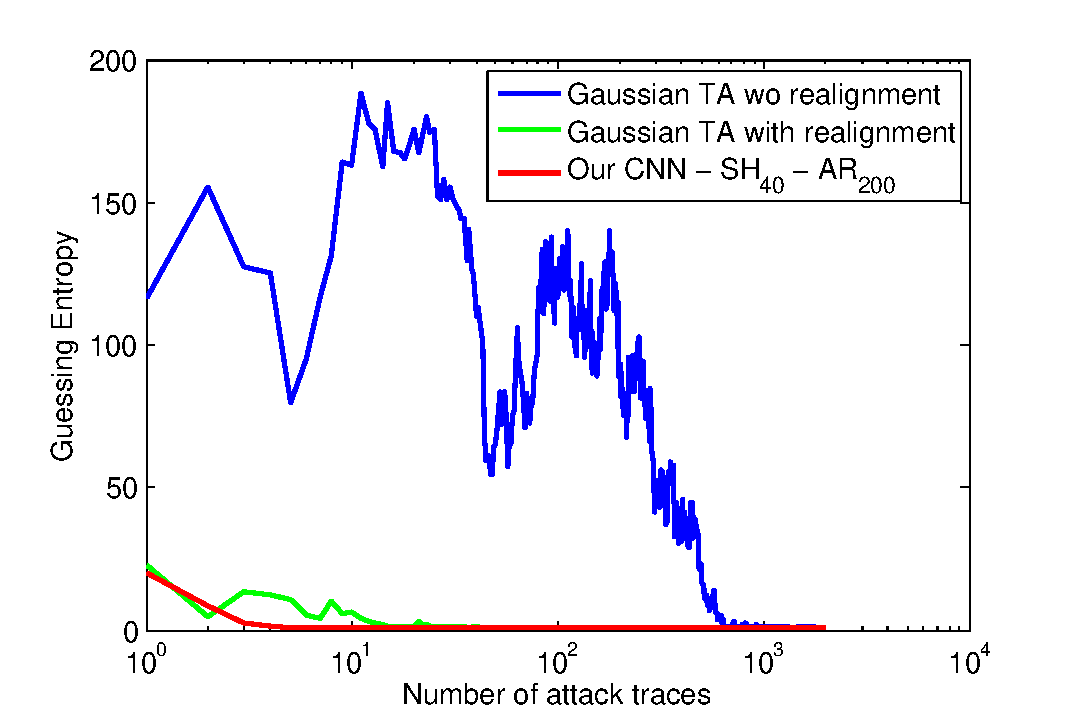
\includegraphics[width=.5\textwidth]{../Figures/CHES2017/results_low_jitter_new.pdf} 
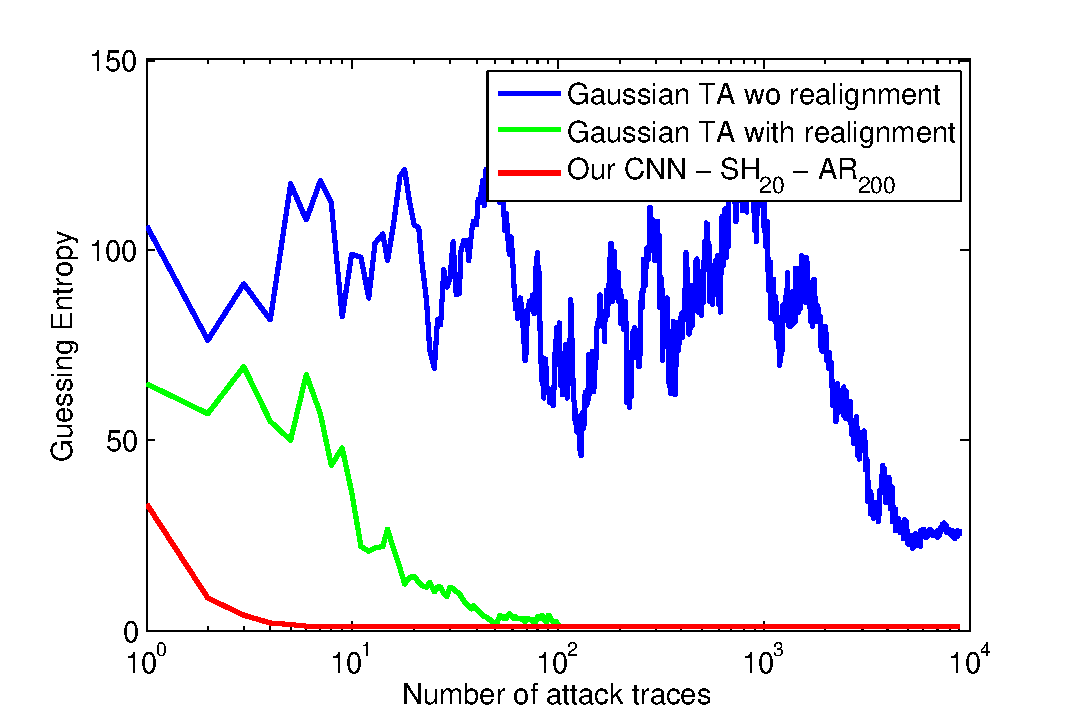
\includegraphics[width=.5\textwidth]{../Figures/CHES2017/results_high_jitter_new.pdf} 
\caption[Comparison between a Gaussian template attack, with and without realignment, and our CNN strategy, over the  \emph{DS\_low\_jitter} and the  \emph{DS\_high\_jitter}.]{Comparison between a Gaussian template attack, with and without realignment, and our CNN strategy, over the  \emph{DS\_low\_jitter} (left) and the  \emph{DS\_high\_jitter} (right).}\label{fig:compareTA}
\end{figure}

\paragraph*{Exp�riences en cas de contremesure mat�rielle r�elle}

\begin{table}
\centering
\begin{tabular}{|c|c|c|c|c|c|c|c|}
\multicolumn{8}{c}{}\\
\hline
\multicolumn{2}{|c|}{} & \multicolumn{2}{c|}{$\mathrm{SH}_{0}\mathrm{AR}_{0}$} & \multicolumn{2}{c|}{$\mathrm{SH}_{10}\mathrm{AR}_{100}$} & \multicolumn{2}{c|}{$\mathrm{SH}_{20}\mathrm{AR}_{200}$} \\ \hline
$a$        & $b$       & 35.0\%                     & 1.1\%                    & 12.5\%                      & 1.5\%                      & \textbf{10.4\%}             & \textbf{2.2\%}             \\ \hline
$c$        & $d$       & 1.2\%                      & 137                      & 1.3\%                       & 89                         & \textbf{1.8\%}              & \textbf{54}                \\ \hline
\end{tabular}

\caption{R�sultats de l'attaque par CNN sur carte � puce prot�g�e par jitter.}\label{tab:res_AES}
\end{table}

Les r�sultats prometteurs du contexte simul� se retrouvent aussi dans le dernier sc�nario d'exp�rience, o� la cible est une impl�mentation mat�rielle de l'AES sur composant s�curis�e moderne. L'impl�mentation est prot�g� par un effet de jitter sur l'horloge. Comme montr� dans le Tableau~\ref{tab:res_AES}, l'attaque par CNN est efficace et les techniques DA mitigent le surapprentissage du r�seau en am�liorant l'attaque. Dans ce contexte nous comparons la strat�gie classique, qui consiste � effectuer une attaque template suite � une technique de r�-alignement et au choix minutieux des PoIs, et la strat�gie par CNN sans r�-alignement ni extraction explicite de caract�ristiques. L'attaque par CNN se montre l�g�rement plus efficace m�me en absence de pr�-traitements. 

\begin{figure}
    \centering
    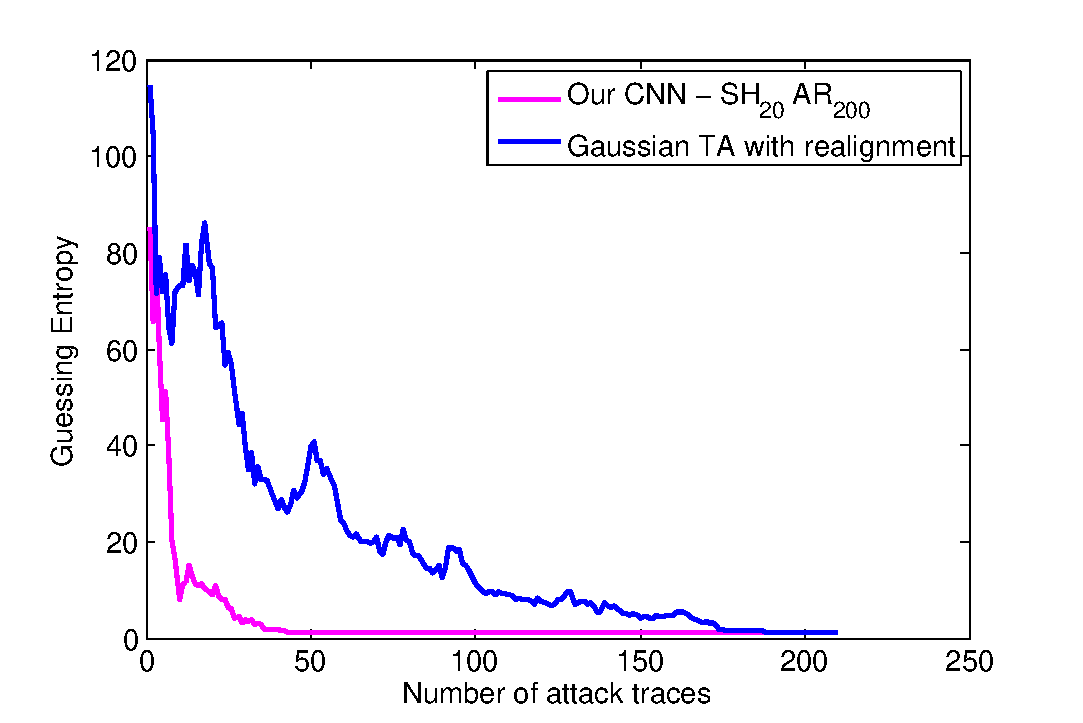
\includegraphics[width=.5\textwidth]{../Figures/CHES2017/TA_CNN_smartcard.pdf} 
     \caption{Comparaison entre l'attaque template gaussienne avec r�-alignement, et la strat�gie par CNN, sur carte � puce prot�g�e par jitter.}\label{fig:TA_smartcard}
\end{figure}


\section{Conclusions et Perspectives}\label{sec:conclusions}

Dans cette th�se, nous nous sommes concentr�s sur les attaques par profilage. L'opportunit� de caract�riser les fuites de la cible ouvre les portes �  des approches optimales, permettant l'estimation des distribution de probabilit� conditionnelle n�cessaire �  identifi� la cl� secret par maximum \emph{a-posteriori}. Cependant, l'effort d'estimer les distributions de probabilit� de donn�es largement multivari�es est emp�ch� par la \emph{mal�diction de la dimension}. Nos premiers effort se sont consacr� au d�veloppement de technique de r�duction de dimension, et nous avons propos� deux contributions �  ce sujet. Dans une troisi�me contribution nous abordons la mal�diction de la dimension �  l'aide mod�les par r�seaux neuronaux. \\

Le fil rouge de cette th�se a �t� la croissante conscience du fait que les probl�mes pratiques auxquelles on est confront�s dans le domaine des attaques par canaux auxiliaires sont presque identiques dans d'autres domaines d'application, et l'approche par apprentissage automatique s'est av�r� gagnant dans plusieurs d'entre eux. Nous avons particip� alors �  une conversion des probl�matiques SCA, en passant d'une approche statistique classique, �  une approche par apprentissage automatique. Nous croyons que cette conversion m�rite d'�tre poursuivie dans le future. Une prochaine �tape devrais \^etre la d�finition d'une t\^ache d'apprentissage automatique qui soit parfaitement adapt� aux contexte des attaques avanc�e: en effet, jusqu'�  pr�sent, nous avons utilis� des outils d�di�s �  la t\^ache de la classification, qui ne correspond pas parfaitement �  ce type d'attaque. Des m�triques et des crit�res d'optimisation sp�cialis�s pour les SCA devrait �tre propos�s. Deuxi�mement, dans l'optique de renforcer la r�sistance des dispositifs s�curis�, des m�thodes d'analyse des mod�les d'apprentissage profond menant �  la r�ussite des attaque sont n�cessaires, afin d'interpr�ter l'action de ces mod�les, identifi� les caract�ristiques des signaux qui plus contribuent �  leur r�ussite, retrouver et �  terme �liminer les vuln�rabilit�s de l'impl�mentation qui ont permis �  ces caract�ristiques de fuir �  travers les canaux auxiliaires. 

\bibliographystyle{plain}
\bibliography{all_my_bib}



\end{document}
